\documentclass[11pt, a4paper, fleqn, final]{book}
\usepackage[linesnumbered]{algorithm2e}
\usepackage{amsfonts}
\usepackage{amsmath}
\usepackage{amsthm}
\usepackage{chngpage}
\usepackage{cite}
\usepackage{fullpage}
\usepackage{hyperref}
\usepackage{subfig}
\usepackage{thmtools}
\usepackage{tikz}

\newcommand{\specialcell}[2][l] {
  \begin{tabular}[#1]{@{}l@{}}#2\end{tabular}
}

\newtheorem{definition}{Definition}

\begin{document} 

\begin{titlepage}
    \begin{center}
    \vspace*{1cm}

    \huge
    \textbf{RDMA-Based Implementation of BDD Operations for Multicore Clusters}

    \vspace{0.5cm}
    \LARGE
    Research Topics

    \vspace{1.5cm}

    \Large
    \textbf{Wytse Oortwijn}

    \vfill

    \vspace{0.8cm}

    
\includegraphics[width=0.4\textwidth]{images/university.png}

    \large
    Formal Methods and Tools\\
    University of Twente\\
    Netherlands\\
    October 27, 2014
    \end{center}
\end{titlepage}
\tableofcontents

\chapter{Introduction}
This document will contain a project plan for the graduation project of Wytse Oortwijn. This project will attempt to implement BDD operations for multicore clusters. 

\section{Project Title}
RDMA-Based Implementation of BDD Operations for Multicore Clusters.

\section{Project Committee}
The project committe will consist of the following members.
\begin{itemize}
	\item prof.dr. J.C. van de Pol
	\item dr. S.C.C. Blom
	\item T. van Dijk MSc
\end{itemize}

\section{Keywords}
Multi-core programming, Distributed programming, Binary Decision Diagrams, Performance, High Performance Computing, Heterogeneous programming.

\section{Abstract (is old, needs to be rewritten...)}
In the field of program validation one often wants to show that a software program satisfies its requirements. One way of verifying a software program is to generate all reachable program states and check if one of those states is faulty. This important process is known as reachability analysis, as the program is analysed based on all reachable states. It often happens that a program contains so many states that they do not fit into the memory of a (single) computer. This problem is known as the state space explosion problem. Several techniques have been used to minimize this problem. One of these techniques is known as distributed computing, in which the combined resources of a network of computers is used.

One of the biggest bottlenecks of distributed verification and distributed model checking is the network latency. In the last couple of years a lot of research has been done on high-performance distributed computing by using RDMA (Remote Direct Memory Access) to increase throughput and decrease the latency of a network. The idea of RDMA is that a computer can directly read and write into the memory of another computer, while not invoking the CPU on that computer. As a result, multiple distributed key-value stores have been designed (for example FaRM and Pilaf) that can handle up to 75 million network operations per second. 

The goal of this project is to check if RDMA can be used to increase the performance of several distributed verification algorithms, like reachability analysis. By reducing the latency and increasing the throughput of the network, one can considerably speedup distributed computations, perhaps even to the point where parallel and distributed computations can effectively be combined to create heterogenous algorithms. The second goal of the project is to check if parallel and distributed computations can effectively be combined by using RDMA to reduce communication overhead.

\section{Structure}
This document is structured as follows...
\chapter{Motivation}

Model checking is an important tool in software verification. Model checking can be used check if the model of a software system meets its requirements. A model checker can be implemented in various ways, one of which is symbolically \cite{mcmillan1993symbolic, clarke1996symbolic}. Rather than explicitly maintaining states, a symbolic model checker stores the state space as a Boolean formula, represented as a \emph{Binary Decision Diagram (BDD)}. The main advantage of such a representation is that a small Boolean function can potentially represent a large number of states, thus giving an efficient representation of the state space. Symbolic model checking has already been widely used as a verification tool and a fair number of symbolic model checkers already exist \cite{cimatti2000nusmv, marrying}. 

\section{Early Work}
In the early 90's a lot of research has been done on parallel BDD manipulation using massively parallel computers \cite{BDDNOW:parallel_bdd_package, 545652, Stornetta96implementationof, BDDNOW:parallel_bdd_package}. Most work was designed for SIMD machines and vector machines. Researches experimented with different ways to partition work, including BFS, DFS, nested DFS, and hybrid DFS/BFS. In the late 90s research attention shifted towards distributed BDD manipulation. At that time, a network of workstations was the most affordable and best available parallel platform, which motivated the research for distributed BDD manipulation \cite{BDDNOW:parallel_bdd_package}. Experimental results pointed out that very large BDDs could be manipulated due to the aggregated memory of the network, but speedups were not obtained. This was mainly due to network latency, which was the major performance bottleneck. The best results were obtained by the BDD package BDDNOW \cite{BDDNOW:parallel_bdd_package}, which only achieved some speedup when the sequential implementation ran out of main-memory and disk-based storage was used instead.

After the 90s research attention shifted towards the use of BDDs in shared and distributed memory rather than parallel or distributed manipulation of BDDs.

\section{Recent Work}
Hardware changed significantly during the last decade. At the time of writing, parallel hardware is widely available and specialized high performance network interconnects like Infiniband are just as affordable as standard Ethernet hardware. This justifies a renewed attempt to parallelize and distribute BDD operations. One example of this is Sylvan \cite{sylvan_multicore_bdd}, an implementation of parallel BDD operations by using a lockless hash table and a work stealing framework. Sylvan obtained impressive speedups.

This research project attempts to implement BDD operations on a cluster of multicore machines using RDMA-enabled hardware. By doing that, BDD operations can potentially be designed that scale both across the number of CPU cores and the number of participating machines. To our knowledge, this has never been done before.

\section{Project Relevance}
One of the main problems of model checking today is the \emph{state space explosion} problem. A state space explosion occurs when the amount of information the model checker has to examine does not fit into the available memory. Fighting the state space explosion problem is important, because the amount of information that model checkers have to examine also grows every year. 

There are several ways to tackle this problem, including state space reduction and state space minimization techniques \cite{pater2011partial, blom2005distributed}. The use of BDDs is one of such techniques, since it allows a compact representation of the state space. Nonetheless, the state space explosion problem still exists. 

Another way to tackle the state space explosion problem is to increase the available hardware resources. This can be either the increase in memory, the increase in CPU power or both. Manycore computers are very expensive, whereas a cluster of workstations could be cheaper, depending on the size of the cluster.

Earlier attempts to use a cluster for BDD manipulations have shown that larger BDDs can be constructed, compared to BDD construction on a single machine. On the other hand, speedup is only achieved when the single machine ran out of memory \cite{BDDNOW:parallel_bdd_package}. Still, it is justifiable to reconsider the use of multicore clusters for BDD manipulation, because of the recent hardware advances. If this research succeeds, larger model checking problems can be solved in less time, depending on how well the implementation scales along the different hardware resources. Also other verification algorithms can benefit from this research since they too may scale well across a cluster of machines by applying the same ideas.

The third potential of this research project is the development of heterogeneous algorithms for software verification. It is nowadays possible to use RDMA at the GPU level, so it might be possible to create RDMA-based BDD operations that run anywere, including the GPU \cite{gpudirect}. The development of such algorithms is highly relevant in the field of High Performance Computing, and this research project could potentially form the basis for such development.

To our knowledge, the use of RDMA to implement BDD operations on multicore clusters has never been done before.
\chapter{Detailed Approach}

\textit{This section provides research questions, as well as project goals, assumptions, project risks, deliverables, and the activities that are to be performed during the research project.}

\section{Research Questions}
This research project attempts to implement BDD operations for multicore clusters. Implementing them is not trivial, since ideally both CPU and memory capacity of all participating clusters has to be utilized as efficiently as possible. A perfect solution would split work perfectly across the participating processes such that every processing element only needs to access its own local memory. This however cannot easily be achieved, if possible at all. So the first step in this research project is to find out how to deal with this problem. This raises the following three research questions.

\begin{enumerate}
	\item[Q.1]{\textit{How can BDDs be spread over all participating clusters so that the memory of all clusters is used efficiently?}}
	\item[Q.2]{\textit{How can work be partitioned such that every participating process can work as efficiently as possible?}}
	\item[Q.3]{\textit{How can load-balancing be implemented such that the number of network operations is minimized?}}
\end{enumerate}

An answer to these three research questions is given in this report. The goal of the graduation project is to implement and benchmark the BDD operations based on the related work given in this report. Benchmarking is done to test the efficiency of the implementation. The following research questions need to be answered after the implementation and benchmarking phase phase.

\begin{enumerate}
	\item[Q.4]{\textit{How well does the implementation scale across the number of participating CPU cores?}}
	\item[Q.5]{\textit{How well does the implementation scale across the number of participating machines?}}
	\item[Q.6]{\textit{How can the scalability of the implementation be improved?}}
\end{enumerate}

If time permits the result of research question \textit{Q.6} can be used to make the implementation more efficient. This introduces another iteration of implementation and benchmarking (which requires the measurement plan to be re-applied). Also the answers given to the research questions can be adjusted, based on the results found in the second iteration. If time runs short, improving the implementation can be marked as future work.

At the end of the research project a conclusion must be given based on the experimental results, which answers the following main research question. 

\begin{enumerate}
	\item[Q.7]{\textit{Can BDD operations be implemented to perform efficiently on a cluster of multicore machines?}}
\end{enumerate}

Note that \textit{performing efficiently} means utilizing the available hardware resources efficiently. Efficiency is something that can be measured, so a relevant answer to this question can be given in the conclusion of the research project.

\section{Goals and Objectives}
The primary goal of this research project is to create an efficient implementation for BDD operations on multicore clusters that scales well across the number of processes and the number of participating clusters. 

The second goal is to create a paper out of the results obtained from the research. The relevance of these results has already been discussed in the motivational part of this report.

The third goal, which is a personal goal, is to try to obtain a PhD funding during or after the graduation project in order to continue working on heterogeneous algorithms.

\section{Methods and Techniques}
The programming language C is used to create the implementation. MVAPICH2-X 2.1a in combination with OpenSHMEM is used as a hybrid PGAS/MPI communication model. For work stealing, the Scioto framework is used. The BDD operations are simply adjusted versions taken from the multicore BDD package Sylvan.

Benchmarking the communication model can be done by simply sending and receiving one-sided RDMA operations. The distributed hash table can be microbenchmarked with the \emph{YCSB} benchmark \cite{cooper2010benchmarking}. The work stealing implementation can be tested by running a parallel version of the recursive Fibonacci algorithm. The implementation of the BDD operations can be benchmarked by using the entire \emph{BEEM} database \cite{pelanek2007beem}.

\section{Assumptions}
For this research project it is assumed that a cluster of machines, connected via Infiniband, is available for experimental use at the University of Twente. It is also assumed that MVAPICH2-X 2.1a and OpenSHMEM can be installed on the cluster, so that a hybrid PGAS/MPI model can be created. 

\section{Risks}
If MVAPICH2-X 2.1a can not be installed on the cluster, an alternative framework for PGAS/MPI has to be used. This would be a problem, since MVAPICH2-X 2.1a is, to our observation, the best framework for the hybrid PGAS/MPI model on Infiniband hardware. There are not many other frameworks that support the PGAS/MPI model. We could attempt to use UPC \cite{upc} or OpenSHMEM \cite{openshmem} without MVAPICH2-X 2.1a and use only PGAS. The MPI part can then be done with another message passing framework. This however has impact on the performance of the implementation, since MVAPICH2-X 2.1a is very fast.

If OpenSHMEM can not be installed, UPC can be used instead (and the other way around), so we have two alternatives for the PGAS part. Suppose that OpenSHMEM and UPC both can not be installed, then PGAS can not be used and the project has to switch to bare RDMA instead.

The researchers of FaRM \cite{farm} found out that performance decreased significantly when increasing the amount of RDMA-exposed memory. This is because the Infiniband NIC caches page tables. When the amount of exposed memory increases, the cache runs full and the NIC needs to fetch more page tables over the PCI bus. The researchers solved this by using a low-level package called PhyCo (currently unmaintained and declared dead) to increase page sizes to 2GB. This could also happen to our implementation, so we start the implementation phase by testing if RDMA works properly when scaling the amount of exposed memory. 

\section{Prerequisites}
Before starting with the graduation project, MVAPICH2-X 2.1a in combination with OpenSHMEM or UPC must be installed on the cluster connected by Infiniband. If this can not be done for some reason, the risk plan described above has to be executed.

\section{Activities}
The following activities are to be performed during the research project.

\begin{itemize}
	\item Performing a literature study to find out how BDD operations can efficiently be implemented on a cluster of multicore machines.
	\item Implementing an RDMA-based lockless distributed hash table on PGAS.
	\item Microbenchmarking the distributed hash table.
	\item Implementing a work stealing protocol that works on a cluster of multicore machines.
	\item Microbenchmarking the work-stealing protocol.
	\item Presenting the results obtained from the experimental phase in an FMT lunch meeting presentation.
	\item Implementing the BDD operations on top of the distributed hash table.
	\item Benchmarking the implementation of the BDD operations.
	\item If time permits, implementing some of the possible improvements found during the experimental phase.
	\item Finishing the master thesis.
	\item Presenting the master thesis.
	\item Writing the paper containing implementation details and experimental results.
\end{itemize}

\section{Deliverables}
The activities described in the previous section result in the following deliverables.

\begin{enumerate}
	\item A literature study in which related work is discussed and research questions \textit{Q.1}, \textit{Q.2}, and \textit{Q.3} are answered.
	\item A small benchmark to test the latency and throughput of the one-sided RDMA operations.
	\item An RDMA-based distributed hash table that scales well across the available memory of all participating nodes.
	\item A report in which the performance of the distributed hash table is evaluated. This report is the result of microbenchmarking the hash table.
	\item An implementation of the BDD operations that makes use of the distributed hash table.
	\item An report that evaluates the performance of these BDD operations. This report is the result of the experimental phase of the research project.
	\item A conclusion of the experimental phase.
	\item A lunch meeting presentation in which the outcome of the experimental phase, as well as the project itself is presented to the other members of the research group.
	\item A master thesis covering all elements discussed above in this summation.
	\item A master thesis presentation.
	\item A paper in which the implementation and the obtained results are given.
\end{enumerate}
\chapter{Project Planning}

\textit{This section contains planning constraints, a description of the different project phases and the actual project planning.}

\section{Planning Constraints}
The following constraits apply to the project planning.

\subsection{Time Constraint}
The project consists of two parts, namely the Research Topics part and the graduation project part. The Research Topics part takes about 10EC and the graduation project part takes 30EC in total. Every European Credit (EC) stands for 28 hours, so the total time for Research Topics is $10*28 = 280$ hours and for the graduation project $30 * 28 = 840$ hours.

The graduation project has to be completed strictly within half a year, which is 26 weeks. The research topics does not have a fixed time constraint. This time constrait can be elevated a bit, but this requires permission from the project committee. 

\subsection{Unavailability due to Work}
During the research project, Wytse is available for four days a week. This means that Wytse is unavailable one day a week and this extends the length of the graduation project to $1.2 * 26 \approx 32$ weeks.

\subsection{Research Honours Programme}
Wytse is planning to participate in the Research Honours program, which takes an extra $20EC$ if he succeeds. This causes the graduation project to take $50EC$ in total.

\subsection{Winter and Summer Holidays}
The winter holidays, which are two weeks, are excluded from the planning. In case the project takes $50EC$ or more, it will span the summer holidays. In that case the summer holidays are also excluded from the planning.

\subsection{Starting date}
We make use of the fact that the Research Topics phase does not have a fixed deadline. The prerequisite for starting the project is that software for PGAS/MPI is installed on the cluster, so we do not start with the project until the software is installed. We plan to start the project on November 24, 2014.

\subsection{Date of Completion}
The current date of completion is July 17, 2015. This date can change due to the research honours programme. 

\section{Project Phases}
Below are the different project phases and milestones planned throughout the graduation project. Also a short indication is given of the time it takes to complete the phase.

\subsection{Microbenchmarking RDMA}
One of points mentioned in the project risks section of this report is the possible performance drop when increasing the amount of RDMA-exposed memory. This needs to be tested as early as possible, so the project starts by microbenchmarking the performance of RDMA.  

\subsection{Implementing and Microbenchmarking the Distributed Hash Table}
Developing the distributed hash table on top of MPI/PGAS takes about a month to complete. Microbenchmarking the implementation and discussing the results takes about two weeks. If the experimental results disappoint, some extra time is needed to deal with problems in the implementation.

\subsection{Implementing and Microbenchmarking the Work Stealing Framework}
Implementing and testing work stealing also takes a month in total. The scalability of the work stealing framework has to be tested, since it gives an indication of the scalability of the BDD operations. This can be done by performing a microbenchmark. If the benchmark results dissapoint, another work stealing framework can be tried or changes can be applied to the framework.

\subsection{Implementing and Benchmarking the BDD operations}
After having a good implementation of the distributed hash table and a work stealing protocol, the BDD operations have to be implemented. This will take roughly three weeks and benchmarking the BDD operations takes about two weeks.

\subsection{Finishing the Thesis}
Some time is reserved just for finishing the master thesis. Note that part of the writing process can be done during the other phases. We are planning to also release a paper on the results of this research project, so also the paper is finished during this phase.

\section{Planning}
The project planning is presented in Table \ref{tab:planning1} and \ref{tab:planning2}.

\begin{table}[ht]
	\begin{adjustwidth}{-.5in}{-.5in} 
	\centering
	\begin{tabular}{| c | c | c | l |}
		\hline
		\textbf{\specialcell{Project\\week}} & \textbf{\specialcell{Date\\(begin - end)}} & \textbf{\specialcell{Nr. of\\hours}} & \textbf{Project activities} \\ 
		\hline \hline
		1 & \specialcell{Nov 24, 2014\\Nov 28, 2014} & 32 & Implementing the DHT, \textit{32 hours} \\ \hline
		2 & \specialcell{Dec 1, 2014\\Dec 5, 2014} & 32 & Implementing the DHT, \textit{32 hours} \\ \hline
		3 & \specialcell{Dec 8, 2014\\Dec 12, 2014} & 32 & \specialcell{Implementing the DHT, \textit{16 hours}\\Writing a chapter on the DHT, \textit{16 hours}} \\ \hline
		4 & \specialcell{Dec 15, 2014\\Dec 19, 2014} & 32 & \specialcell{Finishing the first version of the DHT, \textit{8 hours}\\Finishing the chapter on the DHT, \textit{24 hours}} \\ \hline

		5 & \specialcell{Jan 5, 2015\\Jan 9, 2015} & 32 & Microbenchmarking the DHT, \textit{32 hours} \\ \hline
		6 & \specialcell{Jan 12, 2015\\Jan 16, 2015} & 32 & Microbenchmarking the DHT, \textit{32 hours} \\ \hline
		7 & \specialcell{Jan 19, 2015\\Jan 23, 2015} & 32 & \specialcell{Adjusting the DHT, \textit{16 hours}\\Writing a chapter with benchmark conclusions, \textit{16 hours}} \\ \hline
		8 & \specialcell{Jan 26, 2015\\Jan 30, 2015} & 32 & \specialcell{Adjusting the DHT, \textit{8 hours}\\Finishing the chapter on benchmark conclusions, \textit{24 hours}} \\ \hline \hline

		9 & \specialcell{Feb 2, 2015\\Feb 6, 2015} & 32 & Implementing work-stealing, \textit{32 hours} \\ \hline
		10 & \specialcell{Feb 9, 2015\\Feb 13, 2015} & 32 & Implementing work-stealing, \textit{32 hours} \\ \hline
		11 & \specialcell{Feb 16, 2015\\Feb 20, 2015} & 32 & Implementing work-stealing, \textit{32 hours} \\ \hline 
		12 & \specialcell{Feb 23, 2015\\Feb 27, 2015} & 32 & \specialcell{Implementing work-stealing, \textit{16 hours}\\Writing a section on work-stealing, \textit{16 hours}} \\ \hline
		13 & \specialcell{Mar 2, 2015\\Mar 6, 2015} & 32 & \specialcell{Implementing work-stealing, \textit{16 hours}\\Writing a section on work-stealing, \textit{16 hours}} \\ \hline 
		14 & \specialcell{Mar 9, 2015\\Mar 13, 2015} & 32 & \specialcell{Testing and finishing work-stealing, \textit{16 hours}\\Finishing the section on work-stealing, \textit{16 hours}} \\ \hline\hline

		15 & \specialcell{Mar 16, 2015\\Mar 20, 2015} &32 & \specialcell{Implementing BDD operations, \textit{16 hours}\\Writing a chapter on BDD operations, \textit{16 hours}} \\ \hline
		16 & \specialcell{Mar 23, 2015\\Mar 27, 2015} & 32 & \specialcell{Implementing BDD operations, \textit{16 hours}\\Writing a chapter on BDD operations, \textit{16 hours}} \\ \hline
		17 & \specialcell{Mar 30, 2015\\Apr 3, 2015} & 32 & \specialcell{Finishing the BDD operations, \textit{8 hours}\\Writing a chapter on BDD operations, \textit{24 hours}} \\ \hline
	\end{tabular}
	\end{adjustwidth}
	\caption{Graduation project planning, first part, weeks 1 to 17.}
	\label{tab:planning1}
\end{table}

\begin{table}[ht]
	\begin{adjustwidth}{-.5in}{-.5in} 
	\centering
	\begin{tabular}{| c | c | c | l |}
		\hline
		\textbf{\specialcell{Project\\week}} & \textbf{\specialcell{Date\\(begin - end)}} & \textbf{\specialcell{Nr. of\\hours}} & \textbf{Activities} \\ 
		\hline \hline
		18 & \specialcell{Apr 6, 2015\\Apr 10, 2015} & 32 & Benchmarking the BDD operations, \textit{32 hours} \\ \hline
		19 & \specialcell{Apr 13, 2015\\Apr 17, 2015}  & 32 & \specialcell{Benchmarking the BDD operations, \textit{24 hours}\\Writing a chapter on benchmark results, \textit{8 hours}} \\ \hline
		20 & \specialcell{Apr 20, 2015\\Apr 24, 2015}  & 32 & \specialcell{Benchmarking the BDD operations, \textit{16 hours}\\Writing a chapter on benchmark results, \textit{16 hours}} \\ \hline
		21 & \specialcell{Apr 27, 2015\\May 01, 2015}  & 32 & \specialcell{Finishing benchmarking, \textit{8 hours}\\Finishing the chapter on benchmark results, \textit{24 hours}} \\ \hline \hline

		22 & \specialcell{May 04, 2015\\May 08, 2015} & 32 & \specialcell{Writing a concept thesis, \textit{32 hours}} \\ \hline
		23 & \specialcell{May 11, 2015\\May 15, 2015} & 32 & \specialcell{Writing a concept thesis, \textit{32 hours}} \\ \hline
		24 & \specialcell{May 18, 2015\\May 22, 2015} & 32 & \specialcell{Writing a concept thesis, \textit{8 hours}\\Writing the paper, \textit{24 hours}} \\ \hline
		25 & \specialcell{May 25, 2015\\May 29, 2015} & 32 & \specialcell{Writing a concept thesis, \textit{8 hours}\\Writing the paper, \textit{24 hours}} \\ \hline
		26 & \specialcell{Jun 01, 2015\\Jun 05, 2015} & 32 & \specialcell{Writing a concept thesis, \textit{16 hours}\\Writing the paper, \textit{16 hours}\\Handing in the concept thesis} \\ \hline \hline

		27 & \specialcell{Jun 08, 2015\\Jun 12, 2015} & 32 & \specialcell{Creating a presentation, \textit{32 hours}} \\ \hline
		28 & \specialcell{Jun 15, 2015\\Jun 20, 2015} & 32 & \specialcell{Preparing the presentation, \textit{8 hours}\\ Lunch-meeting presentation, \textit{2 hours}\\Finishing the thesis, \textit{20 hours}} \\ \hline \hline

		29 & \specialcell{Jun 22, 2015\\Jun 26, 2015} & 32 & \specialcell{Finishing the thesis, \textit{32 hours}} \\ \hline
		30 & \specialcell{Jun 29, 2015\\Jul 03, 2015} & 32 & \specialcell{Finishing the thesis, \textit{8 hours}\\Finishing the paper, \textit{24 hours}} \\ \hline

		31 & \specialcell{Jul 06, 2015\\Jul 10, 2015} & 32 & \specialcell{Finishing the thesis, \textit{16 hours}\\Adjusting the presentation, \textit{16 hours}} \\ \hline
		32 & \specialcell{Jul 13, 2015\\Jul 17, 2015} & 32 & \specialcell{Handing in Thesis\\Preparing the presentation, \textit{24 hours}\\Presenting the thesis, \textit{8 hours}} \\
		\hline
	\end{tabular}
	\end{adjustwidth}
	\caption{Graduation project planning, second part, weeks 18 to 32.}
	\label{tab:planning2}
\end{table}

\subsection{Planning Risks}
The most important aspect of this project is the creation and evaluation of a distributed hash table that uses PGAS and one-sided RDMA operations where possible. If the implementation of the distributed hash table takes longer than expected for some reason, the implementation of BDD operations can be omitted. If needed, the paper can also be written after the graduation project.

The implementation of the work stealing protocol can be done ourselves, but if time runs short Scioto \cite{dinan2008scioto} can be used instead. Scioto is a work-stealing framework especially designed for the PGAS model and exploits locality. 


\chapter{Measurement Plan}

\textit{The research project contains a couple of phases in which measurements are performed. This chapter discusses the experimental setup and the experiments that are to be performed.}

\section{Experimental Setup}
The experiments are performed on ten Intel E5520 dual-core machines connected via an Infiniband network, each with 24GB RAM. The operating system installed on each machine is Ubuntu 14.04 LTS. The Infiniband hardware supports up to 20 Gbps. So the cluster consists of 20 CPU cores and 240GB RAM in total, divided over 10 machines.

Our cluster-based BDD operations can be compared with Sylvan, the multicore parallel BDD package created at the University of Twente. These experiments can be performed on a 48-core machine with 128GB total memory (NUMA), available at the University of Twente. 

\subsection{Changes in the Setting}
It seems that the hardware inventory that is publicly available is outdated, so changes may occur in the hardware setting described above. When this happens, the experimental setup section in this document will be updated accordingly.

\section{Plan of Measurement}
First the the RDMA operations are benchmarked to test for performance drops. Secondly the implementation of the distributed hash table is to be benchmarked to test the effectiveness of the hashing scheme. Then the work stealing framework has to be microbenchmarked to test the effectiveness of load-balacing in a cluster of multicore computers. Finally the implementation of the BDD operations are to be benchmarked.

This section gives a measurements plan for each of these benchmarking phases.

\subsection{Microbenchmarking the RDMA operations}
The first step is to benchmark the one-sided RDMA operations. The researchers of FaRM \cite{farm} found out that performance drops significantly when the amount of memory exposed via RDMA is increased. This is because the NIC caches page tables from main-memory. When the amount of RDMA-exposed memory grows, the number of page tables also grows, which causes the cache to eventually become full. Then more cache pages need to be transfered to the NIC over the PCI bus, which slows performance significantly. 

This could be problematic, because we want to create a distributed hash table that is exposed via RDMA. We are not exactly sure if MVAPICH2-X 2.1a solves this problem, but this can be easily tested by running some small tests. Is performance drops when allocating a lot of memory with RDMA, a trick can be used to increase page sizes (FaRM uses a kernel driver called PhyCo), but we would rather not use such tricks.

The following experiments are to be applied to test one-sided RDMA operations.

\begin{enumerate}
	\item Benchmark the latency of the one-sided \texttt{read}, \texttt{write}, and \texttt{cas} operations by sending a number of RDMA calls to the target machine. Repeat the benchmark for different packet sizes to test the effect of increasing the workload of the RDMA operation.
	\item Benchmark the throughput of the one-sided \texttt{read}, \texttt{write}, and \texttt{cas} operations by sending a number (say, $100.000$) of RDMA operations to another computer. Repeat the benchmark for different packet sizes to test the effect of increasing the workload of the RDMA operation.
	\item Benchmark the throughput and latency of the one-sided \texttt{read}, \texttt{write}, and \texttt{cas} operations by increasing the amount of memory exposed via RDMA. Here it is important to access multiple pages, so use a large number (say, $100.000$) of RDMA operations, distributed uniformly (or otherwise randomly) over the entire block of RDMA-exposed memory. This can optionally be combined by increasing the workload of the operations.
	\item In order to show the significance of one-sided RDMA, some of these experiments could be repeated with a normal TCP connection and the results can be compared to the RDMA-based experiments. If it is to hard to change the code to work with TCP, we could use \emph{RDMA over Converged Ethernet (RoCE)} instead.
\end{enumerate}

We do not put too much time in benchmarking the RDMA-operations, but it is important to know if exposing large blocks of memory with RDMA causes performance drops. That is the real important thing here. Measuring performance and throughput under different workloads gives a good indication of how much of a bottleneck the network latency will be. This is not crucial for the research project, but can be used in performance analysis, estimating research expectations and to give improvements on the implementation.

\subsection{Microbenchmarking the Distributed Hash Table}
After the distributed hash table has been developed, it has to be microbenchmarked. This gives a good performance indication for the BDD operations. Quite some things have to be benchmarked in this phase, since the implementation of a good distributed hash table is the \emph{core component} of the research project. 

First of all, some analysis can be performed to predict the estimated number of network operations that have to be performed by using hash table operations. This can be done by using statistics (i.e. probability theory). We would like to know the following facts, assuming we use the Hopscotch scheme.

\begin{enumerate}
	\item The expected number of items in a neighborhood under different load-factors and with different neighborhood sizes.
	\item The expected number of hash collisions under different load-factors and with different neighborhood sizes.
	\item The expected length of the collisions chain (for more information on collision chains, see the chapter on hash tables) under different load-factors and with different neighborhood sizes.
	\item The probability that a neighborhood gets full.
\end{enumerate}

Together with the experimental results of the RDMA operations, this analysis can for example greatly help us to determine the most efficient neighborhood size. By then we know the performance of RDMA operations under different workloads as well as the expected number of RDMA reads required, so a performance analysis can also be performed.

Secondly we microbenchmark the implementation of the distributed hash table and we compare the results to our theoretical analysis. This forces us to be critical about the experimental results, which is a good thing. The experiments can be performed by using the \emph{YCSB} benchmark \cite{cooper2010benchmarking}, which is a benchmark provided by Yahoo that tests the performance of key-value stores. The following experiments are to be applied.

\begin{enumerate}
	\item The latency of the \texttt{get} and \texttt{put} operations, both locally and remotely (i.e. both on local and remote memory) under different load-factors.
	\item The throughput of the \texttt{get} and \texttt{put} operations, both locally and remotely (i.e. both on local and remote memory) under different load-factors. 
	\item The average number of RDMA operations performed during a \texttt{get} or \texttt{put} operation under different workloads (i.e. packet sizes).
	\item The number of times collision chaining occurs upon a \texttt{put} operation (i.e. the element does not fit into the corresponding neighborhood, so an item from the neighborhood has to be replaced), under different load-factors.
	\item The average number of items in a neighborhood under different load-factors.
\end{enumerate}

Similarly to the RDMA operation experiments, these experiments can be repeated with TCP (or otherwise RoCE) to show the sigificance of one-sided RDMA. The results on these experiments can be used to improve the implementation of the distributed hash table. If we can improve on the number of RDMA operations, this has to be done. Minimizing the number of RDMA operations is \emph{crucial} for both scalability and speedup of any application built on top of the hash table. 

\subsection{Microbenchmarking the Work Stealing Framework}
The implementations of the parallel BDD operations described in \cite{sylvan_multicore_bdd, dijk2012parallelization} use a work stealing framework to exploit fine-grained parallelism. Work stealing is also involved in this research project. We are planning to use the Scioto framework \cite{dinan2008scioto} for work stealing in a PGAS environment. The main challenge of creating a work stealing framework for multicore clusters is to exploit locality. It might be beneficial to prefer task stealing from local process over remote process. We would like to test this. Benchmarking can be performed by using the work stealing version of the Fibonacci algorithm. The following experiments are to be performed.

\begin{enumerate}
	\item The speedup obtained by the work stealing framework by increasing the number of CPU cores on a single machine.
	\item The speedup obtained by the work stealing framework by increasing the number of machines with the restriction that each machine uses only one CPU core.
	\item The speedup obtained by scaling both across the number of CPU cores and the number of machines.
	\item The average number of local steals and remote steals.
\end{enumerate}

These benchmarkes give a good indication of how well parallelization can be applied in a cluster of multicore machines. With these tests we can predict the performance and scalability of the BDD implemenations a bit.

\subsection{Benchmarking the BDD operations}
The BDD operations can be built on top of the distributed hash table and the work stealing platform. If both are implemented properly, implementing BDD operations on top of them is not that hard. All the models of the \emph{BEEM} database \cite{pelanek2007beem} can be used to test the implementation. The following experiments are to be performed.

\begin{enumerate}
	\item The execution time, speedup, and efficiency obtained when increasing the number of CPU cores, while using only a single machine. The results of this experiment can also be used to compare our implementation with other implementations, like Sylvan \cite{sylvan_multicore_bdd}.
	\item The execution time, speedup, and efficiency obtained when increasing the number of machines with the restriction that each machine uses only a single CPU core.
	\item The execution time, speedup, and efficiency obtained by scaling both across the number of CPU cores and the number of machines.
\end{enumerate}

The results of these experiments (and perhaps also the results from earlier experiments) can be used to improve on the implementation. In that case, the plan of measurements must be re-applied. If time runs short, the improvements can be mentioned as future work.

\chapter{Research Expectations}

For the distributed hash table, the Hopscotch hashing scheme is used. This hashing scheme ensures that \texttt{get} operations require only a single one-sided RDMA read to complete due to the Hopscotch invariant. One-sided RDMA operations have a latency of approximately $2 \mu s$, so \texttt{get} operations can be performed in only $2 \mu s$. 

The \texttt{put} operation requires a one-sided read and a \emph{compare-and-swap} operation when there is room left in the neighborhood. Otherwise a collision chain occurs, which requires an additional amount of reads and \emph{compare-and-swap} operations equal to the length of the chain. Perhaps some extra operations for locking are required, but the Channel Adapter handles incoming RDMA messages sequentially, which makes concurrent programming a bit easier. Since \texttt{compare-and-swap} also takes about $2 \mu s$, we expect \texttt{put} operations to complete in about $6 \mu s$ without resolving hash collisions.

The Computed Table needed for the BDD operations is a simplified hash table. Hash collisions are resolved simply by overwriting the colliding bucket. Because of that, both the \texttt{get} and \texttt{put} operations for the Computed Table can be completed in about $2 \mu s$. Because every hash table operation requires only a few microseconds to complete, we expect the implementation of the BDD operations to scale well across a cluster of machines.

Despite the low latency of the hash table operations, we still expect the network latency to become a performance bottleneck. Processors can perform a huge amount of CPU instructions in the time a roundtrip is made with RDMA, so we expect that only a part of the available processing power is used. This implies that multicore scalability would decrease with the number of machines added to the cluster.

This can only be solved by exploiting locality. Luckily, work stealing frameworks that expoit locality can be designed. For example, Scioto \cite{dinan2008scioto} exploits locality by using a priority queue, so that local work is prioritized over remote work. Steal attempts are performed on work with low priority. The quality of locality exploitation is very important to effectively combine parallel and distributed computations. We expect that they can effectively be combined, but perhaps not entirely within this research project. If not, then research can be done in locality exploitation for work stealing.
\chapter{Background Information on Network Communication}

\section{The Infiniband Architecture}
Infiniband is specialized hardware used to construct networks for High-Performance Computing. Infiniband uses all kinds of tricks to achieve very high throughput, including a bidirectional serial bus to keep communication costs as low as possible. In order to support such bus, Infiniband comes with specialized switches and network interface cards (\emph{NICs}). Those interface cards are called \emph{Channel Adapters} in Infiniband terminology. Infiniband is manifactured by Intel and Mellanox and provides hardware for 10, 20, or 40GB bandwidth.

One of the features supported by Infiniband is \emph{Remote Direct Memory Access}, shortened to \emph{RDMA}. By using RDMA one can even further increase throughput. RDMA will be discussed in the next section.

\subsection{Components}
The network structure of Infiniband differs a bit from the standard Ethernet networking model. A device that is connected to an Infiniband network is called a \emph{node}. Two nodes are connected to each other by so-called \emph{Channel Adapters}, which is the Infiniband counterpart of the network interface card used in Ethernet networks. 

\subsection{Queue-based Model}
On top of the Channel Adapters, Infiniband uses a queue-based model. If two nodes need to communicate to each other, a communication channel between them needs to be set up. Here both nodes must create a \emph{Queuing Pair} consisting of a \emph{Sending Queue} and a \emph{Receiving Queue}. These two queues reside in the memory of the Channel Adapter itself and not in main memory. This allowes the Channel Adapter to handle with incoming messages instead of the CPU, so to support RDMA operations.

If a node wants to send a message, it simply places the message on the Send Queue of the Queuing Pair corresponding to the communication channel between the two nodes. The Channel Adapter will pop the message form the queue when it is ready and places it on the Receiving Queue of the receiving node. Then the Channel Adapter of the receiving node can handle the message. 

Completed messages can be placed in the \emph{Completion Queue}. Such queue is present on all nodes and allow workers to be efficiently notified on completed work. 

\subsection{Service Types}
When a Queuing Pair is created, a \emph{Service Type} must be associated to it. The service type determines how a node must respond to incoming messages. There are five types of service types.

\begin{itemize}
	\item The \emph{Reliable Connection (RC)} service type guarantees a reliable data transfer between the two nodes. This means that data is guaranteed to arrive at the destination node. This is done by responding with an Ack or Nak packet after receiving a message, which makes it very similar to a TCP connection. Another effect of Reliable Connection is that packets are delivered in order and that erroneous messages are automatically retransmitted.

	\item \emph{Unreliable Connection (UC)} specifies a connection between two nodes in which data is not guaranteed to arrive. The responding node does not Ack or Nak each request packet. The advantage compared to a Reliable Connection is that less network traffic is generated and throughput is increased, at the cost of possible packet losses. Also erroneous messages will be disposed rather than retransmitted.

	\item In the \emph{Unreliable Datagram (RD)} service type no responses are expected, which makes it very similar to an UDP connection. Multicasts are supported, but RDMA and Atomic operations are not.

	\item \emph{Reliable Datagram (RD)} is similar to \emph{Unreliable Datagram}, but here the responding node does Ack or Nak each request packet. This guarantees that data arrives, thus making the connection reliable.

	\item Finally the \emph{Raw Datagram} connection is supported, which is similar to \emph{Unreliable Datagram}. Here request packets are not interpreted by the receiving nodes. Like in \emph{Unreliable Datagram} RDMA and Atomic operations are not supported. 
\end{itemize}

Table \ref{tab:service_type_capabilities} presents all service types and their capabilities. For this research project both RDMA reads and writes are needed, so either RC or RD has to be used. 

\begin{table}[ht]
	\centering
	\begin{tabular}{| l | c | c | c | c | c |}
		\hline
		\textbf{Operation} & \textbf{UD} & \textbf{UC} & \textbf{RC} & \textbf{RD} & \textbf{Raw} \\ 
		\hline 
		Send/Receive & X & X & X & X & X \\
		RDMA write &  & X & X & X &  \\
		RDMA read &  &  & X & X &  \\
		Atomic operations &  &  & X & X & \\
		Compare and Swap &  &  & X & X & \\
		\hline
	\end{tabular}
	\caption{The different operations enabled by the four service types used in Infiniband.}
	\label{tab:service_type_capabilities}
\end{table}

\subsection{Supported Operations}
Like seen in Table \ref{tab:service_type_capabilities} Infiniband supports several types of operations depending on the service type used. A small list of operations supported by Infiniband is given below.

\begin{itemize}
	\item The standard \emph{Send/Receive} operations just involves the standard sending and receiving of messages. The \emph{Send} operation will put a message on the Receiving Queue of the targetted node and the \emph{Receive} operation will poll the Receiving Queue for incoming messages.

	\item The \emph{one-sided RDMA} operations do only use the Sending Queue of the Queuing Pairs. If a node wants to execute an one-sided RDMA operation, it simply puts such a work item on its Sending Queue. The Channel Adapter will eventually transmit the work item to the targetted node and are directly executed once received.

	\item The \emph{two-sided RDMA} operations are similar to the one-sided ones, but here the Receiving Queue is used. This means that the CPU of the targetted node has to be used to handle incoming packets, but these operations are still faster than the Send/Receive operations since they bypass the kernel. More on RDMA operations is presented in the next chapter.

	\item Some of the service types support \emph{Atomic Operations}. There are two types of atomic operations supported by Infiniband, namely \emph{Compare and Swap (CAS)} and the \emph{Atomic Fetch and Add (AFAD)}. 
\end{itemize}

In addition to these operations Infiniband also supports transactions and multicast operations. 

\subsection{Hardware Costs}
One of the main advantages of Infiniband is that hardware prices are comparable to their Ethernet counterparts. In fact, at the time of writing, Infiniband hardware is even cheaper. This further motivates the use of Infiniband in High-Performance Computing and for performing research in how such hardware can be used to speed-up exiting distributed algorithms.

\subsection{Hardware Availability}
The University of Twente currently has ten computing nodes connected via an Infiniband network. The Infiniband Network used is a 20GB bandwidth version. The computing nodes all have a Dual Intel E5520 processor with a clock speed of 2.27GHz and 24GB of internal memory. This makes a total of twenty processing cores and 240GB of combined internal memory. All nodes run with Open-Suse. 


\section{Remote Direct Memory Access}
One of the most interesting features that comes with Infiniband is \emph{RDMA}, which stands for \emph{Remote Direct Memory Access}. With RDMA a
node can operate on the memory of another node without invoking the Operating System of any of the two nodes. 

\subsection{Zero-Copying}
Normally when sending a packet over a TCP connection the packet is copied several times. First the packet is copied from user memory into kernel memory, then the packet is send across the network, copied in kernel memory of the receiving node and finally copied into user memory. This also includes three context switches.

In RDMA the network stack is completely bypassed, since packets are directly placed on the Sending Queue in the Channel Adapter. The receiving Channel Adapter will either directly execute the message in case of a one-sided operation or place it on the Receiving Queue when a two-sided operation is used. 

This greatly reduces latency and increases throughput of network operations compared to the traditional network stack. 

\subsection{One-Sided RDMA}
One-sided RDMA operations do not invoke the CPU on the targetted node since RDMA messages received are directly executed by the Channel Adapter. The Channel Adapter can directly access main memory, so the Operations System as well as the CPU do not have to be invoked. 

A one-sided RDMA write operation can directly be executed on the targetted machine. A one-sided read operation on the other hand requires the targetted machine to send an answer back to the source node. The answer is then written to the Completion Queue of the source node. 

Because of the full roundtrip, one-sided RDMA reads are slower than RDMA writes, since they do not need a full roundtrip. Some systems completely avoid RDMA reads and only use writes in order to achieve maximal throughput. Such implementations mostly use circular buffers exposed with RDMA to create a message-passing alternative.

\subsection{Two-Sided RDMA}
Like explained earlier, two-sided RDMA operations do use the Receiving Queue of the targetted machines. The workers themselves have to pop work items from the Receiving Queue to process them. This makes two-sided RDMA operations similar to the read and write operations that are supported by Infiniband, but the network stack is still bypassed.

Two-sided operations can be used when the work is more complicated than accessing memory or performing a CAS operation. The targetted node will manually execute the work and most of the benefits of RDMA are still used.

\subsection{RDMA over Converged Ethernet}
A disadvantage of RDMA is that it requires specialized hardware. In order to support RDMA on Ethernet hardware a network protocol called \emph{RDMA over Converged Ethernet}, shortened to \emph{RoCE} is invented. This allowes software systems that are using RDMA to support standard Ethernet hardware. RoCE further increases the motivation to use RDMA in this research project.

By using RoCE the Channel Adapters are replaced by NICs which do not have direct access to main memory. So the CPU has to be invoked for every RDMA operation send over RoCE. On the other hand, RoCE still uses the zero-copy policy and the network stack is still bypassed as much as possible, thus making RoCE faster than most other networking protocols implemented over Ethernet.

\subsection{RDMA over Infiniband}
In order to support RDMA operations on remote memory, the Channel Adapter needs to be aware of the chunks of memory that are RDMA-exposed. So a block of memory can be registered by the Channel Adapter via the Infiniband interface. An RDMA-registered block of memory is called a \emph{Memory Region}. Every such region has a local and a remote address to be used locally and remotely, respectively. The remote addresses can be translated to local addresses by a table lookup in the Channel Adapter. RDMA operations can thus be performed by using the remote addresses. Transmitting the remote addresses to other nodes can be done by using MPI for example.

By registering a memory region at the Channel Adapter, one can also give permissions to that region. Those permissions are managed by a \emph{protection domain}. In a protection domain, one can give node-specific and operation-specific permissions. Every memory region is part of a protection domain.


\chapter{Parallel Programming Models}
In this section different parallel programming models are discussed, together with their advantages and disadvantages.

\begin{figure}
	\centering
	\subfloat[Shared Memory] {
		\input{Tikz/SharedMemory}
		\label{fig:shared_memory}
	}
	$\hspace{36pt}$
	\subfloat[Distributed Memory] {
		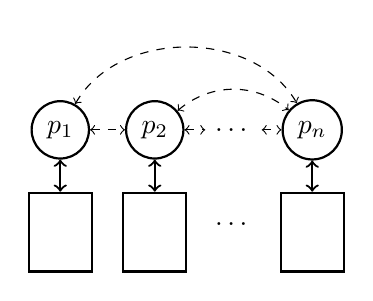
\begin{tikzpicture}
\node[circle, thick, draw] (v1) at (-0.2,0.8) {$p_1$};
\node[circle, thick, draw] (v3) at (1,0.8) {$p_2$};
\node (v7) at (2,0.8) {$\dots$};
\node at (2,-0.4) {$\dots$};
\node[circle, thick, draw] (v5) at (3,0.8) {$p_n$};

\node (v2) at (-0.2,-0.11) {};
\node (v4) at (1,-0.11) {};
\node (v6) at (3,-0.11) {};

\draw[thick] (-0.6,0) rectangle (0.2,-1);
\draw[thick]  (0.6,0) rectangle (1.4,-1);
\draw[thick]  (2.6,0) rectangle (3.4,-1);

\draw[<->, thick]  (v1) edge (v2);
\draw[<->, thick]  (v3) edge (v4);
\draw[<->, thick]  (v5) edge (v6);

\draw[<->, dashed]  (v1) edge (v3);
\draw[<->, dashed]  (v3) edge (v7);
\draw[<->, dashed]  (v7) edge (v5);
\draw[<->, dashed]  (v3) edge [bend left=40 ] (v5) ;
\draw[<->, dashed]  (v1) edge [bend left=60 ] (v5);

\end{tikzpicture}
		\label{fig:distributed_memory}
	}

	\caption{Here $n$ processes $p_1, \dots, p_n$ are displayed in a \emph{Shared Memory} and a \emph{Distributed Memory} setting. Dashed edges represent communication links between processes.}
	\label{fig:shared_distributed_memory}
\end{figure}

\section{Shared Memory Architecture}
In a \emph{Shared Memory Architecture (SMA)}, all processes work in a shared address space, like shown in Figure \ref{fig:shared_memory}. Note that interprocess communication is done implicitly, since every process can access the entire address space.

Since the entire available memory can be accessed via a shared address space, the shared memory model simplifies programming. Algorithms with challenging data dependencies can be modelled elegantly in shared memory. A disadvantage is that data locality is not taken into account, because processes are not aware where data resides. This could bring performance penalties.

\subsection{NUMA}
An example of a shared memory architecture is \emph{Non-Uniform Memory Access (NUMA)}, a model used in computer systems with multiple CPUs. In NUMA every CPU has a local memory and and every CPU can access memory local to other CPUs via a shared address space. Some parts of the address space are on different buses than others, so different parts of the address space may differ in performance. This makes memory accesses non-uniformly.

NUMA is contrasted with \emph{Uniform Memory Access (UMA)}, in which all CPUs share the same physical memory uniformly.

\subsection{SMP}
Another example of shared memory architectures is the \emph{Symmetric Multiprocessing (SMP)} architecture. In SMP all CPUs access memory via the same shared memory bus. Memory-intensive algorithms generally perform better under the NUMA architecture, since the single memory bus in SMP can easily become a performance bottleneck.

\section{Distributed Memory Architecture}
Figure \ref{fig:distributed_memory} shows a \emph{Distributed Memory Architecture (DMA)}. In DMA every process can only access its private memory. When a process needs to access memory that is private to another process, it needs to do so via message passing. This is represented in Figure \ref{fig:distributed_memory} by the dashed edges between processes. 

DMA is widely used to create distributed programs, i.e. programs that run on a cluster of computing machines. Every participating machines has a CPU and main memory, which fits perfectly in the distributed memory model. Machines can send messages to each other via the network. DMA can also be used on a single machine if the available memory is large enough. A popular interface for message passing is the \emph{Message Passing Interface (MPI)}. Applications using the distributed memory model generally use the SPMD programming style.

An advantage of DMA is that data locality is fully exploited, since processes only access local memory. Also programs created with the distributed memory model can easily be distributed across a cluster of machines. Memory management on the other hand is a lot harder, because the available memory is distributed.

\begin{figure}
	\centering
	\subfloat[PGAS] {
		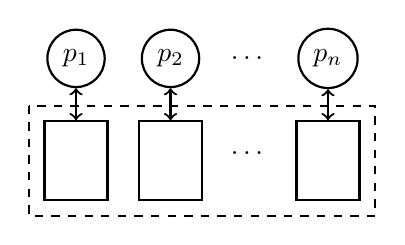
\begin{tikzpicture}
\node[circle, thick, draw] (v1) at (-0.2,0.8) {$p_1$};
\node[circle, thick, draw] (v3) at (1,0.8) {$p_2$};
\node (v7) at (2,0.8) {$\dots$};
\node at (2,-0.4) {$\dots$};
\node[circle, thick, draw] (v5) at (3,0.8) {$p_n$};

\node (v2) at (-0.2,-0.11) {};
\node (v4) at (1,-0.11) {};
\node (v6) at (3,-0.11) {};

\draw[thick] (-0.6,0) rectangle (0.2,-1);
\draw[thick]  (0.6,0) rectangle (1.4,-1);
\draw[thick]  (2.6,0) rectangle (3.4,-1);

\draw[<->, thick]  (v1) edge (v2);
\draw[<->, thick]  (v3) edge (v4);
\draw[<->, thick]  (v5) edge (v6);

\draw[thick, dashed]  (-0.8,0.2) rectangle (3.6,-1.2);
\end{tikzpicture}
		\label{fig:pgas}
	}
	$\hspace{36pt}$
	\subfloat[Hybrid PGAS+MPI] {
		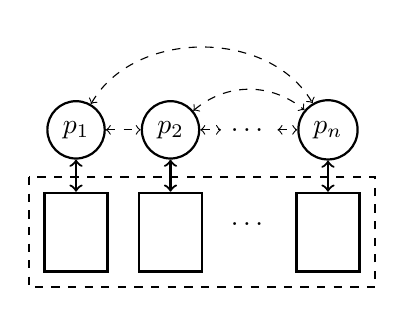
\begin{tikzpicture}
\node[circle, thick, draw] (v1) at (-0.2,0.8) {$p_1$};
\node[circle, thick, draw] (v3) at (1,0.8) {$p_2$};
\node (v7) at (2,0.8) {$\dots$};
\node at (2,-0.4) {$\dots$};
\node[circle, thick, draw] (v5) at (3,0.8) {$p_n$};

\node (v2) at (-0.2,-0.11) {};
\node (v4) at (1,-0.11) {};
\node (v6) at (3,-0.11) {};

\draw[thick] (-0.6,0) rectangle (0.2,-1);
\draw[thick]  (0.6,0) rectangle (1.4,-1);
\draw[thick]  (2.6,0) rectangle (3.4,-1);

\draw[<->, thick]  (v1) edge (v2);
\draw[<->, thick]  (v3) edge (v4);
\draw[<->, thick]  (v5) edge (v6);

\draw[thick, dashed]  (-0.8,0.2) rectangle (3.6,-1.2);

\draw[<->, dashed]  (v1) edge (v3);
\draw[<->, dashed]  (v3) edge (v7);
\draw[<->, dashed]  (v7) edge (v5);
\draw[<->, dashed]  (v3) edge [bend left=40 ] (v5) ;
\draw[<->, dashed]  (v1) edge [bend left=60 ] (v5);
\end{tikzpicture}
		\label{fig:pgas_hybrid}
	}
	\caption{Here $n$ processes $p_1, \dots, p_n$ are displayed in an \emph{PGAS} setting. Every process can access the entire combined memory, of which a small portion is local. The global address spaces are represented by dashed rectangles and the local address spaces by solid rectangles. }
	\label{fig:pgas_hybrid_pgas}
\end{figure}

\section{Partitioned Global Address Space}
The shared and distributed memory models can be combined into a \emph{distrbited shared memory} model. This is shown in Figure \ref{fig:pgas}. Every process has a local memory and all local memories are combined into a single global address space. This model is called \emph{Partitioned Global Address Space (PGAS)}, since the global address space is partitioned by the local memories of the participating processes. This makes PGAS a NUMA architecture.

PGAS combines most of the advantages of both the shared and distributed (SPMD) memory models. Data locality is exploited because every process knows its local memory. PGAS can be used both on a single computer and on a cluster of computers, because of its distributed structure. This simplifies programming systems to scale both parallel and distributed. 

\subsection{Asynchronous Partitioned Global Address Space}
A variant to PGAS is the \emph{Asynchronous Partitioned Global Address Space (APGAS)} model \cite{APGAS}. In APGAS the PGAS model is extended with tasks and task pools. Every node can asynchronously create and execute tasks both locally and remotely. Dynamic load-balancing is automatically applied over tasks. The PGAS model implicitly assumes all processes to run on similar hardware. APGAS has a richer execution framework due to its task-based structure and works well on non-uniform clusters.

\subsection{PGAS and MPI}
A \emph{Hybrid PGAS+MPI} parallel programming model can be used by combining PGAS with the distributed memory model. This is shown in Figure \ref{fig:pgas_hybrid}. In this model processes are able to perform message passing in addition to PGAS. The hybrid model can be used to implement software that does not entirely fit into the PGAS model. Also legacy code written for MPI can benefit from this model.

\subsection{PGAS and RDMA}
If PGAS is used in a distributed setting, it can be combined with RDMA. Every process creates an address space using virtual memory as an abstraction to the entire available memory. Local memory operations can simply be performed and remote operations are translated into one-sided RDMA operations. This makes the combination of RDMA and PGAS a high-performance parallel and distributed platform. 

\section{Parallel Programming Libraries}
This section introduces several parallel programming libraries that can be used in the research project.

\subsection{Message Passing Interface}
The \emph{Message Passing Interface (MPI)} is a popular interface for process communication written in C. With MPI processes can communicate by exchanging messages. MPI is used to create scalable parallel programs, as well as distributed programs.

MPI-3 supports one-sided communication and \emph{Remote Memory Access (RMA)} \cite{conf/sc/GerstenbergerBH13}, so MPI-3 is not longer limited to message passing alone. Many implementations of MPI-3 use RDMA when available to implement the one-sided operations and RMA. MPI also supports the shared memory model \cite{mpi-shared-mem-win}. 

\subsubsection{RMA and RDMA}
The difference between RMA and RDMA is that RDMA requires specialized hardware to directly access remote memory. Remote memory access can still be performed when RMDA-enabled hardware is not available by involving the OS kernel. MPI thus supports the use of remote memory calls without the need of specialized hardware by dropping the requirement of directly accessing remote memory. Many implementations of MPI however do use RDMA when the hardware enables it.

\subsubsection{MVAPICH2}
\emph{MVAPICH2} \cite{mvapich2} is an efficient implementation of MPI-3 for Infiniband hardware. It is efficient in the sense that hardware optimizations are used where possible. MVAPICH comes with a number of variants, one of which is \emph{MVAPICH2-X}, which supports PGAS and the hybrid PGAS/MPI model on Infiniband hardware. This implementation can be used with the PGAS models UPC and OpenSHMEM \cite{implementing_openshmem}. 

\subsubsection{PGAS and GPUs}
Another variant is \emph{MVAPICH2-GDR} \cite{Wang:2011:MOG:1997883.1997893}, which makes use of the GPUDirect RDMA technology \cite{gpudirect}. With MVAPICH2-GDR algorithms can be designed to operate on GPU clusters. It would be possible to design heterogeneous algorithms by combining MVAPICH2-X and MVAPICH2-GDR, but this is future work.

\subsection{PGAS Languages}
A number of PGAS languages exist, including Unified Parallel C (UPC), Co-array Fortran (CAF), Titanium, X10, Chapel, and OpenSHMEM. The languages UPC, CAS, and Titanium are extensions to C, Fortran, and Java, respectively. Since we are not planning to work with Fortran or Java, the languages CAS and Titanium are not discussed. 

\subsubsection{APGAS implementations}
Chapel and X10 are both implementations of the APGAS model \cite{Chamberlain:2007:PPC:1286120.1286123, Charles:2005:XOA:1103845.1094852}. Both are actual programming languages influenced by C++ and Java. These languages provide direct support for PGAS, task management and dynamic task load-balancing. A disadvantage is that the structure of both languages differs from C, so all existing BDD operations written in C have to be rewritten to X10 or Chapel if one of these languages is used. Also interoperability with LTSmin (or other existing tools) could be problematic, so these two languages are not discussed in this research project.

\subsubsection{OpenSHMEM}
OpenSHMEM (Open Shared Memory) is a specification for a standard API for parallel programming in PGAS \cite{openshmem}. Several implementations of OpenSHMEM exist, including an implementation for MVAPICH2-X. The performance of MVAPICH2-X in combination with OpenSHMEM is evaluated in \cite{openshmem_perf_evaluation} and compared to other OpenSHMEM libraries. The experiments were performed on the TACC Stampede cluster \cite{stampede_cluster}. The researchers concluded that this combination delivered best performance and scalability. Especially the atomic and collective operations performed significantly better due to the efficient use of Infiniband hardware. The atomic operations include \texttt{compare-and-swap} and \texttt{fetch-and-add} and the collective operations include \texttt{broadcast}, \texttt{reduce}, \texttt{collect}, and \texttt{barrier}. 

MVAPICH2-X can also be used in combination with UPC. Although this combination is not benchmarked in \cite{openshmem_perf_evaluation}, the benchmarks presented on the MVAPICH2 website show that UPC performs slightly better.

\section{Work Stealing}
Parallelization can be applied by dividing a big problem into smaller tasks so that multiple processes perform work simultaneously. The distribution of these tasks to processes is called \emph{load balancing}. In the ideal case, the work can be split perfectly into $n$ equal parts so that all $n$ processes receive an equal amount of work. In that case a speedup of $n$ can be achieved. However, this can not easily be done in practice, especially when the problem size is initially unknown. A number of different load balancing strategies exist that attempt to maximize speedup.

An efficient method to implement fine-grained task parallelism is \emph{work stealing}. In work stealing each process maintains a local task pool. Processes do not communicate with each other until they run out of tasks. In that case, the process attempts to steal work from other processes, then called \emph{victims}. The program terminates when all processes run out of tasks.

\subsection{Tasks}
A \emph{task} is a small part of a computation that only depends on its own intermediate \emph{subtasks} for its execution. When executing a task, it can create subtasks and later synchronize on those subtasks to complete the execution. Recursive algorithms can very easily be parallelized by using task-based parallelization, possibly in combination with a sort of cache to avoid redundant work. Since BDD operations are defined recursively, task-based parallelization can very well be applied to parallelize BDD operations, like shown in \cite{sylvan_multicore_bdd}.

Many task-based parallel frameworks like Cilk \cite{blumofe1996cilk}, Wool \cite{faxen2009wool}, and Lace \cite{lace} use the operations \texttt{spawn} and \texttt{sync} to spawn new tasks and synchronize on tasks, respectively. The \texttt{spawn} operation creates a new task and every task must be mached with a \texttt{sync} operation, like tasks are stored on a stack. The \texttt{sync} operation waits until the corresponding task completes and retrieves the results from that task. 

\begin{figure}
	\centering
	\begin{algorithm}[H]
		\SetStartEndCondition{ }{}{}%
		\SetKwProg{Fn}{int}{\string:}{}
		\SetKwFunction{fun}{fib}
		\SetKw{KwTo}{in}\SetKwFor{For}{for}{\string:}{}%
		\SetKwIF{If}{ElseIf}{Else}{if}{}{elif}{else}{}%
		\SetKwFor{While}{while}{:}{fintq}%
		\SetKw{test}{in}{}%
		\AlgoDontDisplayBlockMarkers\SetAlgoNoEnd\SetAlgoNoLine%

		\Fn{\fun{$n$}} {
			\textbf{if} $n < 2$ \textbf{return} $n$ \\
			\textbf{return} \texttt{fib}$(n-1)$ + \texttt{fib}$(n-2)$
		}
	\end{algorithm}

	\caption{The original recursive implementation of the Fibonacci function.}
	\label{fig:fib_seq}
\end{figure}

\begin{figure}
	\centering
	\begin{algorithm}[H]
		\SetStartEndCondition{ }{}{}%
		\SetKwProg{Fn}{int}{\string:}{}
		\SetKwFunction{fun}{par-fib}
		\SetKw{KwTo}{in}\SetKwFor{For}{for}{\string:}{}%
		\SetKwIF{If}{ElseIf}{Else}{if}{}{elif}{else}{}%
		\SetKwFor{While}{while}{:}{fintq}%
		\SetKw{test}{in}{}%
		\AlgoDontDisplayBlockMarkers\SetAlgoNoEnd\SetAlgoNoLine%

		\Fn{\fun{$n$}} {
			\textbf{if} $n < 2$ \textbf{return} $n$ \\
			\textbf{spawn}$(\texttt{par-fib}, \ n - 1)$ \\
			\textbf{spawn}$(\texttt{par-fib}, \ n - 2)$ \\
			$r \gets$ \textbf{sync} \\
			\textbf{return} $r \ + $ \textbf{sync}
		}
	\end{algorithm}

	\caption{The implementation of the Fibonacci function that uses fine-grained task-parallelism.}
	\label{fig:fib_par}
\end{figure}

Figure \ref{fig:fib_seq} shows the recursive implementation of the Fibonacci function. This implementation can easily be made parallel by performing the two recursive calls in parallel. Figure \ref{fig:fib_par} shows the same function, but now implemented with fine-grained task-parallelism. The two recursive calls now become subtasks and when both subtasks have completed (i.e. both \textbf{sync} operations yielded a result) the task itself completes. 

\begin{figure}
	\centering
	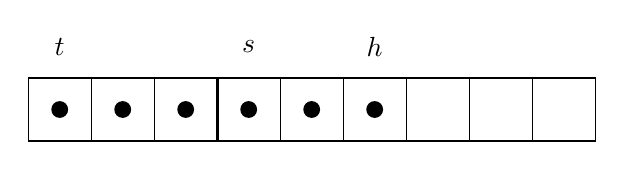
\begin{tikzpicture}[scale=0.8]
\draw[rectangle, draw]  (-1,0) rectangle (0,1);
\draw[rectangle, draw]  (0,0) rectangle (1,1);
\draw[rectangle, draw]  (1,0) rectangle (2,1) node (v1) {};
\draw[rectangle, draw]  (2,0) node (v2) {} rectangle (3,1);
\draw[rectangle, draw]  (3,0) rectangle (4,1);
\draw[rectangle, draw]  (4,0) rectangle (5,1);
\draw[rectangle, draw]  (5,0) rectangle (6,1);
\draw[rectangle, draw]  (6,0) rectangle (7,1);
\draw[rectangle, draw]  (7,0) rectangle (8,1);

\draw[rectangle, very thick, draw]  (2,-0) rectangle (2,1);

\node[circle, fill, draw, inner sep=2pt] at (-0.5,0.5) {};
\node[circle, fill, draw, inner sep=2pt] at (0.5,0.5) {};
\node[circle, fill, draw, inner sep=2pt] at (1.5,0.5) {};
\node[circle, fill, draw, inner sep=2pt] at (2.5,0.5) {};
\node[circle, fill, draw, inner sep=2pt] at (3.5,0.5) {};
\node[circle, fill, draw, inner sep=2pt] at (4.5,0.5) {};

\node at (-0.5,1.5) {$t$};
\node at (4.5,1.5) {$h$};
\node at (2.5,1.5) {$s$};

\end{tikzpicture}
	\caption{The split deque with a head $h$, a tail $t$, and a split point $s$. Here three items are added to the head of the queue and three items to the tail.}
	\label{fig:deque1}
\end{figure}

\begin{figure}
	\centering
	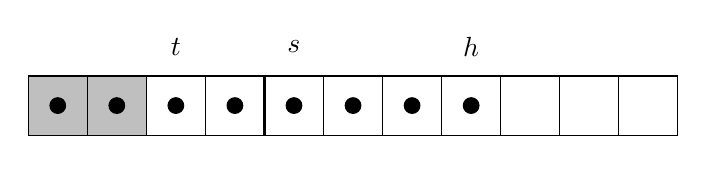
\begin{tikzpicture}[scale=0.75]
\draw[rectangle, color=black, fill=lightgray]  (-1,0) rectangle (0,1);
\draw[rectangle, color=black, fill=lightgray]  (0,0) rectangle (1,1);
\draw[rectangle, draw]  (1,0) rectangle (2,1) node (v1) {};
\draw[rectangle, draw]  (2,0) node (v2) {} rectangle (3,1);
\draw[rectangle, draw]  (3,0) rectangle (4,1);
\draw[rectangle, draw]  (4,0) rectangle (5,1);
\draw[rectangle, draw]  (5,0) rectangle (6,1);
\draw[rectangle, draw]  (6,0) rectangle (7,1);
\draw[rectangle, draw]  (7,0) rectangle (8,1);
\draw[rectangle, draw]  (8,0) rectangle (9,1);
\draw[rectangle, draw]  (9,0) rectangle (10,1);

\draw[rectangle, very thick, draw]  (3,-0) rectangle (3,1);

\node[circle, fill, draw, inner sep=2pt] at (-0.5,0.5) {};
\node[circle, fill, draw, inner sep=2pt] at (0.5,0.5) {};
\node[circle, fill, draw, inner sep=2pt] at (1.5,0.5) {};
\node[circle, fill, draw, inner sep=2pt] at (2.5,0.5) {};
\node[circle, fill, draw, inner sep=2pt] at (3.5,0.5) {};
\node[circle, fill, draw, inner sep=2pt] at (4.5,0.5) {};
\node[circle, fill, draw, inner sep=2pt] at (5.5,0.5) {};
\node[circle, fill, draw, inner sep=2pt] at (6.5,0.5) {};

\node at (1.5,1.5) {$t$};
\node at (6.5,1.5) {$h$};
\node at (3.5,1.5) {$s$};

\end{tikzpicture}
	\caption{The split deque in which every stolen element $x < t$ is made gray. Furthermore every element $x$ with $t < x < s$ belongs to the private part of the deque and every element $x \geq s$ belongs to the public part.}
	\label{fig:deque2}
\end{figure}

\subsection{Split Queues for Work Stealing}
The task pool can be implemented as a concurrent split deque \cite{lace}. A \emph{double ended queue (deque)} is similar to a queue, but has two ends, namely a head and a tail. Items can be \emph{pushed} and \emph{popped} from both ends of the deque. Unlike a normal queue, the deque does not require a LIFO or FIFO ordering. A \emph{split deque} is a deque that has a split point. Figure \ref{fig:deque1} shows an example of a split deque. The split point $s$ determines which part of the deque belongs to the head and which part to the tail. A head pointer $h$ and tail pointer $t$ determines the head and tail elements of the deque, respectively. A \emph{concurrent split deque} uses the \texttt{compare-and-swap} operation to enqueue and dequeue items from the split deque. 

The split deque can be splitted into a public and a private queue, where $s$ determines the border of the two queues. Every element $x < s$ belongs to the public queue and can be stolen by other processes. Every element $x \geq s$ belongs to the private queue and can only be accessed by the process owning the split deque. By stealing a task, the \emph{thief} pops an item from the public part of the \emph{victims} split deque and moves $t$ by using \texttt{compare-and-swap}. Thus every element $x < t$ is stolen. This is shown in Figure \ref{fig:deque2} where every element displayed in gray is stolen. 

The split point $s$ can be changed by the process owning the split deque. Changing $s$ can be done when the private part of the deque becomes empty or when it becomes very big. Thieves are not allowed to change $s$, since it would require an expensive memory fence. Instead, \cite{lace} suggests that a special flag \texttt{splitreq} is maintained by the process owning the split deque. The \texttt{splitreq} can be changed by thieves via \text{compare-and-swap} and the owner can check this flag before performing a \texttt{push} or \texttt{pop} operation. If the flag is set, the process moves $s$ so that the private part of the deque grows. Furthermore, the public part of the deque can also shrink by moving $s$ further into the public part. In that case, it could happen that $s < t$, which would mean that every element in the public part of the deque is already stolen. This can be avoided by using a \emph{memory fence} when shrinking the public queue.

A small improvement to work stealing is given in \cite{lace}, which suggests the use of an \texttt{allstolen} flag. This flag is set by the process owning the queue when it detects that all tasks in the public queue are stolen. Thieves can check this flag before attempting to steal a task, thus avoiding unnecessarily steal attempts. Also the owner can check this flag before shrinking the public queue in order to avoid unnecessarily shrinking.

\subsection{Victim Selection}
When a process needs to perform a \texttt{steal} operation, it needs to somehow find a victim. An obvious stategy is to select a victim randomly. Random victim selection appears to perform stable and has nice theoretical properties \cite{Blumofe:1998:PWS:277858.277939}. A disadvantage of random victim selection is that the size of task pools and the work distribution can fluctuate. This has a negative impact on scalability \cite{dinan2009scalable}. Furthermore a skew in the workload may lead to resources being wasted. 

Note that by stealing tasks, the thief performs work for the victim until the stolen task finishes. Now suppose that the victim steals back from the thief. Then the victim performs a part of the work that was stolen from him. This leads to a semi-random strategy called \emph{leapfrogging} \cite{Wagner:1993:LPT:173284.155354}, in which thieves are selected as victims in the process of victim selection. If there are no thieves, or when the thieves do not have any work in their public queue, a random victim is selected. This strategy ensures that the sizes of the task pools are more predictable. For example, Lace is making use of leapfrogging.

Varisteas et al. \cite{varisteas2014dvs} (published in 2014) introduces \emph{deterministic victim selection}, which removes all randomness. In this strategy each worker has a predefined partially ordered set of possible victims. Task distribution is done via a complex policy that achieves a uniform distribution. The researchers observed better scalability and an average performance improvement of $15\%$ compared to Wool.

\subsection{Implementation}
Simplified algorithms for the \texttt{spawn}, \texttt{sync}, and \texttt{steal} operations are given in \cite{lace}. This paper discusses a concurrent implementation of these operations as well as some improvements, but the simplified versions are enough to discuss the principles of work stealing.

\begin{figure}
	\centering
	\begin{algorithm}[H]
		\SetStartEndCondition{ }{}{}%
		\SetKwProg{Fn}{def}{\string:}{}
		\SetKwFunction{fun}{spawn}
		\SetKw{KwTo}{in}\SetKwFor{For}{for}{\string:}{}%
		\SetKwIF{If}{ElseIf}{Else}{if}{}{elif}{else}{}%
		\SetKwFor{While}{while}{:}{fintq}%
		\SetKw{test}{in}{}%
		\AlgoDontDisplayBlockMarkers\SetAlgoNoEnd\SetAlgoNoLine%

		\Fn{\fun{$t$}} {
			\textbf{self}.taskpool.\texttt{push}($t$)
		}
	\end{algorithm}

	\caption{A simple implementation of \texttt{spawn} that adds a task $t$ to a local task pool \cite{lace}.}
	\label{fig:workstealing_spawn}
\end{figure}

\begin{figure}
	\centering
	\begin{algorithm}[H]
		\SetStartEndCondition{ }{}{}%
		\SetKwProg{Fn}{def}{\string:}{}
		\SetKwFunction{fun}{sync}
		\SetKw{KwTo}{in}\SetKwFor{For}{for}{\string:}{}%
		\SetKwIF{If}{ElseIf}{Else}{if}{}{elif}{else}{}%
		\SetKwFor{While}{while}{:}{fintq}%
		\SetKw{test}{in}{}%
		\AlgoDontDisplayBlockMarkers\SetAlgoNoEnd\SetAlgoNoLine%

		\Fn{\fun{}} {
			$\langle s, t \rangle \gets$ \textbf{self}.taskpool.\texttt{pop}() \\
			\If{$s = $ \textbf{stolen}} {
				\While{$\neg t$.done} {
					\texttt{steal-work}($t.thief$)
				}
				$\langle s', t' \rangle \gets $ \textbf{self}.taskpool.\texttt{pop-stolen}() \\
				\Return{$t'$.result}
			}
			\textbf{return} $t.$\texttt{execute()}
		}
	\end{algorithm}

	\caption{A simple implementation of \texttt{sync} that uses leapfrogging \cite{lace}.}
	\label{fig:workstealing_sync}
\end{figure}

\begin{figure}
	\centering
	\begin{algorithm}[H]
		\SetStartEndCondition{ }{}{}%
		\SetKwProg{Fn}{def}{\string:}{}
		\SetKwFunction{fun}{steal-work}
		\SetKw{KwTo}{in}\SetKwFor{For}{for}{\string:}{}%
		\SetKwIF{If}{ElseIf}{Else}{if}{}{elif}{else}{}%
		\SetKwFor{While}{while}{:}{fintq}%
		\SetKw{test}{in}{}%
		\AlgoDontDisplayBlockMarkers\SetAlgoNoEnd\SetAlgoNoLine%

		\Fn{\fun{$v$}} {
			$t \gets v$.tasks.\texttt{steal()} \\
			\If{$\neg(t = \textbf{none})$} {
				$t$.thief = \textbf{self} \\
				$t$.result = $t$.\texttt{execute()} \\
				$t$.done = \textbf{true}
			}
		}
	\end{algorithm}

	\caption{A simple implementation of \texttt{steal-work} that attempts to steal from a victim $v$ \cite{lace}.}
	\label{fig:workstealing_steal}
\end{figure}

Figure \ref{fig:workstealing_spawn} shows a simple implementation of \texttt{spawn}. The \texttt{spawn} operation receives a task $t$ as a parameter and the operation adds it to the local taskpool of the executing process. 

Figure \ref{fig:workstealing_sync} shows an implementation of the \texttt{sync} operation. This operation simply pops a task $t$ with status $s$ from the task pool and executes it. If $t$ is a stolen task, the process continuously steals work from $t$s thief until $t$ completes, thus performing leapfrogging. 

Figure \ref{fig:workstealing_steal} shows the implementation of the \texttt{steal-work} operation. First the algorithm steals a task $t$ from a victim $v$. Stealing a task is performed by popping a task from the public (shared) part of $v$. If this succeeds, then $t$ is executed.

\subsection{Work Stealing on Parallel Clusters}
We would like to implement work stealing on a cluster of multicore machines in an efficient way. The private deque or the lockless split deque can be used here, especially when PGAS is used as parallel model. In case of a split deque, the shared part of the deque can be exposed via RDMA so that other machines can access it. RDMA supports \texttt{compare-and-swap}, so lockless operations on the shared deque can be implemented. Private deques on the other hand are not registered with RDMA. The hybrid MPI/PGAS model can be used to implement private deques. Stealing can be implemented by message passing, or by using a flag that is registered with RDMA. Other processes can set that flag with a \texttt{compare-and-swap} operation if they want to steal work. The process owning the flag can continously poll that flag and if it is set, give the initiated processes some work.

The main difficulty for work stealing on parallel clusters is the victim selection protocol. Faxén et al. \cite{Faxen:2011:MWS:2016604.2016617} describes \emph{hierarchical victim selection}, which takes the hardware hierarchy into account. The researchers created a work stealing library called HotSLAW that uses the hierarchical victim selection protocol. HotSLAW is a hardware topology aware scheduler and victim selection is performed by first trying to steal on the domain locality level of the thief. By default, HotSLAW performs a number of steal attempts that is equal to the number of CPU cores on that domain level. If stealing fails, the victim selection protocol moves higher into the hardware hierarchy and tries again. 

In addition to hierarchical victim selection, the paper also describes \emph{hierarchical chunk selection}. If a steal attempt needs to be performed in a relatively slow environment (for example, stealing from another machine in the network), it makes sense to steal more work in order to minimize the number of steal attempts. This is less important in a fast environment, for example stealing from another thread on the same machine. The amount of work to steal is dependent on the distance between the thief and the victim. On the topmost level in the hierarchy, the \emph{StealHalf} policy is used, taken from \cite{dinan2009scalable}. On the inner levels of the hierarchy, a fixed-sized chunk is used. In the \emph{StealHalf} strategy half of the work of the victim is stolen. This appears to be very effective when inter-node work stealing is frequent of when the task execution tree exibits burstly behavior. 

The performance of HotSLAW is further improved by performing a cutoff based on the depth of the recursion tree. Usually the amount of work gets smaller when moving deeper into the recursion tree. The effect of a cutoff is that tasks (hopefully) remain relatively big, so thieves receive a lot of work on every successful steal.

Dinan et al. \cite{dinan2009scalable} describes the design of work stealing algorithms for PGAS in combination with RDMA. The paper describes a lockless release operation that moves work from the private part of the split deque to the public part. This makes it possible to perform a release operation concurrently with a steal operation. The paper discusses the \emph{StealHalf} strategy and a trick to abort steals if needed. The paper suggests the use of spinlocks and when attempting to steal work from a process, it can periodically pull metadata from the process to check if there is any work to steal. If not, the steal can be aborted and a steal attempt can be performed on another process.

Vu et al. \cite{6846471} describes an algorithm for \emph{link-heterogeneous work stealing}. The paper describes two strategies, namely \emph{Probablistic Work Stealing (PWS)} and \emph{Adaptive Cluster-aware Random Stealing (ACRS)} and the algorithm tries to combine the two strategies as good as possible. With PWS the probability to select a victim is not uniform, but proportional to the inverse of the distance between the thief and the victim. This causes PWS to privilege stealing over fast links, making it inherently local. With ACRS a remote steal is performed concurrently with several sequential steals on the same domain level. By performing a steal attempt on a remote process, the thief does not have to stay idle, but can concurrently try to steal work from local processes. 

\subsection{Related Work}
Cilk and Wool \cite{blumofe1996cilk, faxen2009wool} are two task-based parallel frameworks. Cilk is a compiler-based framework, since it compiles programs written with Cilk to another form. Wool on the other hand is library-based. Cilk is relatively old (it appeared in 1996), and since the release of Cilk-5 \cite{frigo1998implementation} (appeared in 1998) work stealing can be performed with multiple threads. By performing work stealing, Cilk attempts to steal work from the tail of the victim's queue, hoping to maximize the probability of stealing the task with the maximum amount of work.

Lace \cite{lace} is a task-based parallel C library that uses non-blocking concurrent split deques. Lace also gives an implementation with private deques, because they solve some of the limitations of concurrent split deques. Experiments show that Lace is competitive with Wool and with the private deque algorithm. The paper also describes \emph{extended leapfrogging} that solves chaining problems that can arrise when using normal leapfrogging.

Palirria \cite{varisteas2014palirria} (published in 2014) is a work-stealing scheduling method for nested fork/join parallelism. Palirria comes with multiple implementations, including an implementation that uses the deterministic victim selection method and an implementation that has a resource estimation algorithm, which replaces the victim selection policy.
\chapter{Background Information on Hash Tables}

\textit{In this chapter hash tables and hashing schemes are discussed. In particular, techniques for solving hash collisions are discussed that attempt to minimize the number of memory accesses. Also distributed hash tables are discussed.}

\section{Preliminaries}
This section contains preliminary information on hash tables and hashing strategies.

\subsection{Hash Table}
A \emph{hash table} is a widely used data structure in the field of computer science, since inserting and deleting data can be done with amortized time complexity $\mathcal{O}(1)$ \cite{DBLP:conf/vldb/Litwin80}. A hash table $H = (b_1, \dots, b_n)$ consists of a sequence of buckets $b_i$ usually implemented as an array. We write $b_i = \perp$ if $b_i$ is not occupied and $b_i \in D$ otherwise. We assume that $\perp \not \in D$. The \emph{load-factor} of $H$ is denoted by $\alpha = \frac{m}{n}$, where $m$ is the number of items inserted in $H$, so $m = |\{ b_i \ | \ b_i \in D \}|$.

A hash function $h : D \rightarrow \{ 1, \dots, n \}$ is used to map data from some domain $D$ to one of the buckets of $H$. For some $x,y \in D$ with $x \not = y$ it may happen that $h(x) = h(y)$. This is called a \emph{hash collision}. The hash function $h$ is called a \emph{perfect hash function} if $h$ is injective. Alternatively, $h$ is perfect if $$\forall x, y \in D. x \not = y \implies h(x) \not = h(y)$$ A perfect hash function is thus collision-free. In practice, the domain $D$ is unknown and $|D| \gg n$, so usually $h$ is not perfect. 

A \emph{distributed hash table} is a hash table that is distributed across a network of machines. Part of this research project is to create a distributed hash table.

\subsection{Hash Collisions}
There are two main ways of resolving hash collisions, namely by using \emph{chaining} or \emph{open addressing}. 

\subsubsection{Chaining}
In chaining each bucket $b_i$ is implemented as a linked list. Adding an item $x \in D$ to the hash table simply involves adding it to the linked list $b_{h(x)}$, which takes $\mathcal{O}(1)$ time. Searching and deleting data items requires the linked list to be traversed, which takes $\Omega(n)$ time in worst case. This happens when all items are inserted in the same bucket. In practice the linked lists only contain a couple of items, so finding items is generally fast. The probability of having all items inserted in the same buckets is extemely low.

Also note that with a chaining scheme it can happen that $\alpha > 1$, because every bucket has a variable length. 

Chaining is an easy and effective way to resolve hash collisions, since performance decreases linearly with the load factor. A disadvantage of chaining is that it generates a lot of memory overhead. For every element stored in the hash table an extra pointer is needed. Maintaining linked lists requires dynamic memory allocation, and this works particularly bad in concurrent environments, because it requires a tread-safe memory manager or garbage collector. We expect this to perform even worse in a PGAS environment, because it requires dynamic remote memory allocation. Chaining also has poor cache performance, but this is less important in a distributed setting.

\subsubsection{Open Addressing}
Open addressing is a method to resolve collisions by \emph{probing}. This means that upon a hash collision alternative buckets are being searched, possibly by using an alternative hash function.

There are three main types of probing, which are linear probing, quadratic probing, and double hashing. These three types are discussed below.

\paragraph{Linear Probing.}
One way of dealing with hash collisions is trying the next bucket. This is known as \emph{linear probing}. A linear probing hash function $h' : D \times \mathbb{N} \rightarrow \{ 1, \dots, n \}$ can be derived from $h$ by letting \cite{Cormen:2009:IAT:1614191} 
\begin{equation}
	h'(x, i) = h(x) + ci \ \text{mod} \ n \hspace{36pt} \text{where} \ c \in \mathbb{N}
\end{equation}

Laarman et al. \cite{so73119} uses linear probing to create a lockless hash table that is \emph{cache efficient}. The implementation uses linear probing to walk over a cache line, which the authors called \emph{walking-the-line}.

\paragraph{Quadratic Probing.}
Quadratic probing is similar to linear probing, only the hash sequence increases quadratically rather than linearly. A quadratic hash function can be derived as follows \cite{Cormen:2009:IAT:1614191}.
\begin{equation}
	h'(x, i) = h(x) + c_1 i + c_2 i^2 \ \text{mod} \ n \hspace{36pt} \text{where} \ c_1, c_2 \in \mathbb{N}^+
\end{equation}

In linear probing clustering may occur, which is better avoided with quadratic probing. On the other hand, linear probing makes better use of locality. 

\paragraph{Double Hashing.}
Double hashing uses two independent auxiliary hash functions $h_1, h_2 : D \rightarrow \{ 1, \dots, n \}$ instead of one with $h_1 \not = h_2$. First $h_1$ is used and when a hash collision occurs the combined hash function $h'$ \cite{Cormen:2009:IAT:1614191} is used instead until an empty bucket is found.
\begin{equation}
	h'(x, i) = h_1(x) + ih_2(x) \ \text{mod} \ n
\end{equation}

Note that the interval depends on the data rather than a constant, which gives a good hashing distribution (prevents clustering) at the cost of locality.

\section{Alternative Hashing Strategies}
For designing a distributed hash table it is desirable to reduce the amount of network communication as much as possible. One way of doing that is to exploit data locality as much as possible. This can be quite hard, depending on the system that uses the hash table and the problem domain. Another way is to attempt to limit the number of probes performed after hash collisions. There are various alternative hashing strategies that try to minimize the amount of probes. In this section two of them are discussed.

\subsection{Cuckoo Hashing}
The chaining and probing strategies all have an expected worst-case lookup time worse than $\mathcal{O}(1)$. The expected worst-case complexity for a lookup in a hash table that uses chaining is $\mathcal{O}(\frac{\log n}{\log \log n})$ \cite{Gonnet:1981:ELL:322248.322254}. The expected numer of probes when using a probing scheme is $\frac{1}{1 - \alpha}$. Only a perfect hashing scheme achieves a trivial constant worst-case complexity.

\emph{Cuckoo Hashing} \cite{Pagh01cuckoohashing, Pagh:2004:CH:1006424.1006426} is an open address hashing scheme that achieves constant lookup and deletion time and expected constant insertion time. The Cuckoo Hashing scheme uses two independent hashing functions $h_1, h_2 : D \rightarrow \{ 1, \dots, n \}$ with $h_1 \not = h_2$ instead of one. Furthermore the buckets of $H$ contain at most one element. Some Cuckoo hashing variants require two seperate hash tables $H_1, H_2$ to be used, so that $h_i$ is only applied to $H_i$ for $i \in \{ 1, 2 \}$. Cuckoo hashing can also be used with only one table. 

Another advantage of Cuckoo hashing is that it can handle very large load-factors. It is also possible to generalize Cuckoo hashing to use $k$ hash functions $h_1, \dots, h_k : D \rightarrow \{ 1, \dots, n \}$ with $k > 2$ instead of using only two hash functions. Cuckoo hashing with more than two hash functions permits higher load-factors and collisions are less likely to occur.

\subsubsection{Cuckoo Operations}
The idea of Cuckoo hashing is that by inserting some data element $x \in D$ is inserted in either $b_{h_1(x)}$ or $b_{h_2(x)}$. It may happen that both buckets are occupied. In that case the data element $y \in b_{h_1(x)}$ is thrown out to make place for $x$. Then $x$ is placed into $b_{h_1(x)}$ and the insertion algorithm is recursively applied to $y$. When the number of recursive calls meets a certain treshold, the hash table could be rehashed by using two new hash functions, or an error could be thrown. As an effect, every lookup operation requires at most two calls. Checking whether $x \in D$ is in $H$ can be done by checking if $x \in b_{h_1(x)}$ or if not by $x \in b_{h_2(x)}$. This also holds for the delete operation.

\begin{figure}
	\centering
	\subfloat[The \texttt{lookup} algorithm.] {
		\begin{algorithm}[H]
			\SetKwFunction{fun}{lookup}
			\SetKwProg{Fn}{def}{\string:}{}
			\SetStartEndCondition{ }{}{}%
			\AlgoDontDisplayBlockMarkers\SetAlgoNoEnd\SetAlgoNoLine%

			\Fn{\fun{$H, x$}} {
				$(b_1, \dots, b_n) \gets H$\\
				\Return{$b_{h_1(x)} = x \vee b_{h_2(x)} = x$}
			}
		\end{algorithm}
		\label{alg:cuckoo_lookup}
	}
	
	\subfloat[The \texttt{insert} algorithm \cite{Pagh:2004:CH:1006424.1006426}.] {
		\begin{algorithm}[H]
			\SetStartEndCondition{ }{}{}%
			\SetKwProg{Fn}{def}{\string:}{}
			\SetKwFunction{fun}{insert}
			\SetKw{KwTo}{in}\SetKwFor{For}{for}{\string:}{}%
			\SetKwIF{If}{ElseIf}{Else}{if}{}{elif}{else}{}%
			\SetKwFor{While}{while}{:}{fintq}%
			\SetKw{test}{in}{}%
			\AlgoDontDisplayBlockMarkers\SetAlgoNoEnd\SetAlgoNoLine%

			\Fn{\fun{$H, x$}} {
				\If{$lookup(H, x)$} {
					\Return{x}
				}
				$(b_1, \dots, b_n) \gets H$ \\
				$x' \gets x$ \\
				\For{$i \gets 1$ \textbf{to} $treshold$} {

					$b_{h_1(x')} \leftrightarrow x'$ \\
					\textbf{if} $x' = \perp$ \textbf{return} $x$

					$b_{h_2(x')} \leftrightarrow x'$ \\
					\textbf{if} $x' = \perp$ \textbf{return} $x$

				}
				$\texttt{rehash}()$ \\
				$\texttt{insert}(H, x)$
			}
		\end{algorithm}
		\label{alg:cuckoo_insert}
	}

	\caption{Here the \texttt{lookup} and \texttt{insert} algorithms for Cuckoo hash tables are presented. The $\leftrightarrow$ operator denotes the \texttt{swap} operator that swaps the two given operands.}
\end{figure}

Algorithm \ref{alg:cuckoo_lookup} shows the implementation of the \texttt{lookup} algorithm. The \texttt{lookup} algorithm simply checks if $x$ is in one of the buckets corresponding to $h_1(x)$ and $h_2(x)$. At most two memory calls are made due to short-circuit evaluation. When used in a distributed environment, it is possible to retrieve the corresponding buckets asynchronously, thereby improving latency and throughput of the hash table.

The implementation of the \texttt{insert} function is given in Algorithm \ref{alg:cuckoo_insert}. The $\leftrightarrow$ operator used in \texttt{insert} is the swap operator, which swaps the values of the two operands. First \texttt{lookup} is called to test if $x$ is already inserted in $H$. If not, then \texttt{insert} tries to insert $x$ in bucket $b_{h_1(x)}$ by using the swap operator. If $x \not = \perp$, then the algorithm moves to $b_{h_2(x)}$. This construction creates a chain of swaps with a maximal length of $treshold$. The algorithm terminates when $\perp$ is encountered in the chain. When the $treshold$ is reached, the algorithm either rehashes the table (which is the case in Algorithm \ref{alg:cuckoo_insert}) or throws an exception.

\subsubsection{Complexity of the \texttt{insert} Operation}
Assuming that $treshold = \mathcal{O}(n)$ the expected number of iterations in the \texttt{insert} swapping chain is bounded by $\mathcal{O}(1 + \frac{1}{\epsilon})$, where $\epsilon > 0$ is some constant \cite{Pagh:2004:CH:1006424.1006426}. Furthermore the probability that the \texttt{rehash} procedure is called is $\mathcal{O}(\frac{1}{n^2})$.

The \texttt{rehash} procedure simply rehashes all keys using new hash functions and re-inserts all inserted data items. The expected cost of the \texttt{rehash} procedure is $\mathcal{O}(n)$ and the amortized expected cost per insertion is $\mathcal{O}(\frac{1}{n})$. The small probability of the \texttt{rehash} procedure being called implies that the \emph{variance} of the insertion time is constant.

\subsubsection{Experimental results}
In \cite{pilaf} a distributed hash table is implemented as part of an RDMA-based key-value store named Pilaf. The hash table is using a 3-way Cuckoo hashing variant that uses three hash functions. The researchers concluded that the average and maximal number of probes with 3-way cuckoo hashing is $1.6$ and $3$, respectively. The average and maximal number of probes for linear probing is $2.5$ and $213$, respectively. 

Other comparisons between hashing strategies were hard to find. It would be a good idea to test several hashing strategies during the microbenchmarking or analytical phase, since hashing strategies are generally easy to implement. Perhaps analysing them first would be better, since we do not know exactly how complex the PGAS implementation becomes. 

\subsubsection{Bucketized Cuckoo Hashing}
One of the variants on Cuckoo hashing is called \textit{$(k, l)$-Cuckoo Hashing} \cite{180323}. This variant uses $k$ hash functions instead of two and every bucket has $l$ \emph{slots}. Data elements can then be placed on one of the $l$ slots. The \texttt{lookup} operation simply tests if $x$ is on any of the $kl$ slots. The \texttt{insert} operation tries to insert $x$ in any of the $l$ slots before continuing the swap chain. Note that standard Cuckoo hashing is equal to $(2, 1)$-Cuckoo hashing. 

The $(k, l)$-Cuckoo hashing variant has a high space efficiency ($>90\%$ according to \cite{180323}). Also the number of probes may decrease. Combining $(k, l)$-Cuckoo hashing with RDMA could be interesting, since $l$ buckets can be accessed by performing a single RDMA operation. The authors of \cite{pilaf} pointed out that $(2, 4)$-Cuckoo hashing could be very efficient. 

A slight disadvantage is that the probes are slightly larger, since $l$ buckets have to be read. Thus the RDMA operations also become a bit larger. Furthermore, \texttt{compare-and-swap} operations can perfectly be used to implement the swapping operator when $(k, 1)$-Cuckoo hashing is used. This is not immediately the case when $(k, l)$-Cuckoo hashing is used with $l > 1$. This can be fixed by giving each slot a locking flag, so that slots can be locked first and then be accessed. 

\subsubsection{Related Work}
Nguyen et al. \cite{nguyen2014lock} (2014) presents a \emph{lock-free} Cuckoo hashing algorithm that uses \texttt{compare-and-swap}. The researchers also improved the \texttt{insert} algorithm. They found out that during the relocation process data items are temporarily removed from the hash table during each swap. Also, a naive implementation of the relocation process requires the entire collision chain to be locked. The researchers solved this by reversing the collision chain. First an empty slot is searched for by recursively moving into the chain. When found, it is immediately claimed via \texttt{compare-and-swap}. Then a sequence (equal to the chain length) of swaps can be scheduled. These swaps can be done concurrently, again by performing \texttt{compare-and-swap} operations. 

Furthermore, because two buckets can simultaniously being accessed by the \texttt{insert} operation, it is possible that duplicate values occur in the hash table (so the case in which $x$ is inserted in both $b_{h_1(x)}$ and $b_{h_2(x)}$ concurrently). This is solved in the \texttt{lookup} operation by testing for duplicate values. This implies that short-circuit evaluation cannot be applied. In a distributed setting this means that extra RDMA accesses are necessary, which impacts performance.

Li et al. \cite{Li:2014:AIF:2592798.2592820} (2014) presents algorithmic improvements for fast concurrent cuckoo hashing. The researchers used fine-grained locking and tried to minimize the size of the critical sections. Also a locking scheme for the insertion chain is presented. Furthermore a \emph{Hardware Transactional Memory (HTM)} is used to further increase performance.

Kim et al. \cite{enhanced_chained_cuckoo_hashing} (2014) presents an improved chained hashing method and Cuckoo hashing method optimized for modern hardware. The new chaining method uses the size of the CPU cache lines to allocate nodes, so to reduce the number of cache misses. Also changes to pointers in the linked lists are made using \texttt{compare-and-swap}. The new Cuckoo hashing variant is bucketized and the size of each bucket is equal to the size of a CPU cache line. The \texttt{compare-and-swap} operation is used where possible. 

\subsection{Hopscotch Hashing}
Another hashing scheme with expected constant insertion time is \emph{Hopscotch Hashing} \cite{hopscotch}. Hopscotch uses a single hash function $h : D \rightarrow \{ 1, \dots, n \}$ and every bucket is assigned to a \emph{neighborhood}. A neighborhood can be seen as a virtual bucket, spanning over multiple buckets in $H$. Every neighborhood has a fixed size $k > 1$. The neighborhood of bucket $b_i$, denoted by $N(b_i)$, is $b_i$ itself together with the next $k - 1$ buckets, so $N(b_i) = (b_i, \dots, b_{i + k - 1})$. Hopscotch hashing maintains the invariant that every data element $x \in D$ is stored within $N(b_{h(x)})$.

\begin{figure}
	\centering
	\begin{algorithm}[H]
		\SetStartEndCondition{ }{}{}%
		\SetKwProg{Fn}{def}{\string:}{}
		\SetKwFunction{fun}{lookup}
		\SetKw{KwTo}{in}\SetKwFor{For}{for}{\string:}{}%
		\SetKwIF{If}{ElseIf}{Else}{if}{}{elif}{else}{}%
		\SetKwFor{While}{while}{:}{fintq}%
		\SetKw{test}{in}{}%
		\AlgoDontDisplayBlockMarkers\SetAlgoNoEnd\SetAlgoNoLine%

		\Fn{\fun{$H, x$}} {
			$(b_1, \dots, b_n) \gets H$ \\
			$(b'_i, \dots, b'_j) \gets N(b_{h(x)})$ \\

			\For{$p \gets i$ \textbf{to} $j$} {
				\textbf{if} $x \in b_p$ \textbf{return} $true$
			}

			\Return{$false$}
		}
	\end{algorithm}
	\label{fig:hopscotch_lookup}
	\caption{The \texttt{lookup} algorithm used in Hopscotch hashing.}
\end{figure}

Figure \ref{fig:hopscotch_lookup} shows the \texttt{lookup} algorithm for Hopscotch hashing. The algorithm calculates $h(x)$ and checks if $x$ is inserted in $b_{h(x)}$ or in any of the $k - 1$ following buckets. The \texttt{lookup} function returns $true$ if and only if $x \in N(b_{h(x)})$ due to the Hopscotch invariant. Note that \texttt{lookup} works a bit like linear probing, so the CPU cache is used efficiently. If Hopscotch is used in combination with RDMA, $N(b_{h(x)})$ can be obtained by performing only one RDMA operation. 

The \texttt{insert} algorithm for Hopscotch is a bit harder compared to \texttt{lookup} and is not presented in this report. Algorithmic details are given in \cite{hopscotch}. The idea is that if $b_{h(x)} = \perp$, then $b_{h(x)} \gets x$. Otherwise every bucket in $N(b_{h(x)})$ is tried. If every bucket of $N(b_{h(x)}) = (b_i, \dots, b_j)$ is occupied, the algorithm tries to move $b_j$ to another bucket in order to make place for $x$. It does that by placing $b_j$ in an empty bucket in $N(b_j)$. If all buckets in $N(b_j)$ are also filled, the algorithm can either do the same trick recursively, resize and rehash the table or throw an exception, depending on the requirements of the application.

The \texttt{rehash} algorithm is quite easy and is also not discussed in this report. \texttt{reshash} simply chooses a new hash function and re-inserts all data items inserted in $H$.

\subsubsection{Algorithmic Complexity}
The only two functions that really matter for the research project are \texttt{insert} and \texttt{lookup}, so the \texttt{remove} function is not discussed. Table resizing is also not used, because the sized of the distributed hash table is fixed for best performance. Resizing has a negative influence on the overal performance, so it is not discussed further.

The \texttt{lookup} function clearly has a complexity of $\Theta(k)$, where $k$ is the size of the neighborhood. Since $k$ is constant, the \texttt{lookup} function has a constant complexity. 

According to \cite{hopscotch} the expected number of entries tested in the \texttt{insert} function before an open slot is found is at most $\frac{1}{2} \big (1 + \frac{1}{(1 - \alpha)^2} \big )$. Since $\alpha < 1$ the formula is constant, thus the expected computation time of \texttt{insert} is also constant. If $\alpha = 0.5$ then the expected number of entries tested is $2.5$ and for $\alpha = 0.9$ it is $50$, so choosing the right size for $k$ is important, especially when RDMA is involved.

The \texttt{rehash} function simply has a complexity of $\mathcal{O}(m)$, where $m$ is the number of data items inserted in $H$.

\subsubsection{Experimental Results}
The performance of Hopscotch is compared to chained hashing, linear probing, and Cuckoo hashing in \cite{hopscotch}. The researchers concluded that Hopscotch scales better than chained hashing along CPU cores (the other hashing schemes are not included in the multicore test results). Note however that a lock-based chaining scheme is used, which may have a negative influence on the performance of the chaining schemes. 

The probability of probing for an empty slot, with length bigger then $k$ is $\alpha^{k - 1}$ \cite{hopscotch}. The researchers concluded by experimentation that no resizing occured with $\alpha = 0.8$ and $k = 32$, because $\alpha^{k - 1} = \big ( \frac{8}{10} \big )^{31} \approx 0.000990$. This is good enough to work with in practice.

The sequential throughput tests show that Hopscotch performs best, even when the load-factor becomes very high (i.e. $\alpha > 0.9$). A suprising observation is that the Cuckoo hashing scheme stops before $\alpha$ reaches $0.4$, so it could not handle high load-factors. 

\subsubsection{Related Work}
Dragojevic et al. \cite{farm} created a memory distributed computing platform that uses RDMA. They implemented a distributed hash table with the Hopscotch hashing scheme on top of the platform. It appears that large neighborhoods perform badly with RDMA because the read operation gets large. Small RDMA operations perform significantly better than large RDMA operations and with $k = 32$ (which is done in \cite{hopscotch}) the RDMA reads become 2 KB in size. 

The researchers changed the algorithm a bit and designed the \emph{chained associative hopscotch hashing} algorithm, which achieves good balance between size and the number of RDMA calls. With chained associative Hopscotch, the \texttt{lookup} algorithm requires only $1.04$ RDMA reads on average with $k = 8$ and $\alpha = 0.9$. Cuckoo hashing requires $3.2$ RDMA operation on average with $\alpha = 0.75$, but perhaps bucketized Cuckoo hashing can do better. An explanation of the algorithm is given in \cite{farm}, but pseudocode is not included.

\subsection{Bloom filters}
A \emph{Bloom Filter} \cite{dharmapurikar2003longest} is a probablistic data structure used to test if some element is part of a set. Bloom filters generally have two operations, which are \texttt{test} and \texttt{add}. The \texttt{test} operation tests if a data item is a member of the set and \texttt{add} marks the data item as part of the set. Bloom filters are very space-efficient, but the \texttt{test} operation has a probability of producing \emph{false positives}. This means that \texttt{test} sometimes returns true when given some data item that is not part of the set. \emph{False negatives} however cannot occur. 

A Bloom filter is implemented as a bit-vector $B = \langle v_1, \dots, v_p \rangle$ of length $p$ together with $k$ hash functions $h_1, \dots, d_k : D \rightarrow \{ 1, \dots, p \}$ that map data elements from some domain $D$ to one of the $p$ bits in $B$. The implementation of the \texttt{test} and \texttt{add} operations are very simple.

\begin{figure}
	\centering
	\begin{algorithm}[H]
		\SetStartEndCondition{ }{}{}%
		\SetKwProg{Fn}{def}{\string:}{}
		\SetKwFunction{fun}{add}
		\SetKw{KwTo}{in}\SetKwFor{For}{for}{\string:}{}%
		\SetKwIF{If}{ElseIf}{Else}{if}{}{elif}{else}{}%
		\SetKwFor{While}{while}{:}{fintq}%
		\SetKw{test}{in}{}%
		\AlgoDontDisplayBlockMarkers\SetAlgoNoEnd\SetAlgoNoLine%
		
		\Fn{\fun{$V$, $x \in D$}} {
			$\langle v_1, \dots, v_p \rangle \gets V$ \\
			\For{$i \gets 1$ \textbf{to} $k$} {
				$v_{h_i(x)} = 1$
			}
		}
	\end{algorithm}

	\caption{The implementation of the \texttt{add} operation used in Bloom filters.}
	\label{fig:bloom_add}
\end{figure}

\begin{figure}
	\centering
	\begin{algorithm}[H]
		\SetStartEndCondition{ }{}{}%
		\SetKwProg{Fn}{def}{\string:}{}
		\SetKwFunction{fun}{test}
		\SetKw{KwTo}{in}\SetKwFor{For}{for}{\string:}{}%
		\SetKwIF{If}{ElseIf}{Else}{if}{}{elif}{else}{}%
		\SetKwFor{While}{while}{:}{fintq}%
		\SetKw{test}{in}{}%
		\AlgoDontDisplayBlockMarkers\SetAlgoNoEnd\SetAlgoNoLine%

		\Fn{\fun{$V$, $x \in D$}} {
			$\langle v_1, \dots, v_p \rangle \gets V$ \\
			\For{$i \gets 1$ \textbf{to} $k$} {
				\textbf{if} $v_{h_i(x)} = 0$ \textbf{return $false$}
			}
			\Return{\textbf{true}}
		}
	\end{algorithm}

	\caption{The \texttt{test} operation used in Bloom filter.}
	\label{fig:bloom_test}
\end{figure}

Figure \ref{fig:bloom_add} shows the implementation of the \texttt{add} operation. The \texttt{add} operations simply flips all bits corresponding to $h_1(x), \dots, h_k(x)$ to one. Figure \ref{fig:bloom_test} shows the implementation of the \texttt{test} function. This function simply checks if all bits corresponding to $h_1(x), \dots, h_k(x)$ are set to one. If one of these bits is zero, then the algorithm returns $false$. False negatives do not occur, since the \texttt{add} operation would have set all $k$ bits to one if it was inserted. However it may happen that all $k$ bits are set to one, but $x$ has never been inserted. In that case the implementation returns $true$, which is false positive.

\subsubsection{Related Work}
Song et al. \cite{song2005fast} used bloom filters to speed up lookups in hash tables in order to minimize the number of expensive (external) memory accesses in network processing algorithms. Before an expensive lookup is performed in external memory, a bloom filter is queried in internal memory first to test if the data element is in the hash table. If the data element is not in the bloom filter, the expensive lookup operation does not have to be performed, since false negatives do not occur. If the data element is in the bloom filter (possibly the result of a false positive), the lookup is performed. The paper describes an extension to the \texttt{test} operation called the \emph{exact match lookup} that helps the hash table lookup to find the data, thus further reducing the number of memory calls. 

Kirsch et al. \cite{kirsch2006less} shows that the number of hash function $k$ can be reduced to two without affecting the performance. The idea is that two hash function $h_1, h_2$ can be used to create new hash functions $g_i(x) = h_1(x) + ih_2(x)$. The researchers showed that the asymptotic false positive probability does not increase by using only two hash functions.

\subsubsection{Bloom filters and PGAS}
It might be possible to reduce the number of RDMA operations performed on the distributed hash table by using bloom filters. Every participating machine creates a bit-vector in their partition in PGAS (in local memory), on top of their partition of the distributed hash table. Then every \texttt{lookup} operation first checks if the data item is in the bloom filter and every \texttt{insert} operation inserts the data item in the bloom filter. Depending on the hashing scheme used, the improvements describes in \cite{song2005fast, kirsch2006less} can be used to further improve the efficiency of the algorithm.

This would not work, since inserts performed by a process are not inserted in the Bloom filter owned by other processes, so false negatives do occur. It would be possible with an RDMA-based Bloom filter, but this would only increase the amount of RDMA calls.

\section{Distributed Hash Tables}
A \emph{Distributed Hash Table (DHT)} is a hash table that is distributed across a network of machines. By creating a DHT the combined available memory of every machine in the network can be used. DHTs can be implemented in various ways, depending on the programming model used.

If a shared memory architecture is used, then the hash table can simply be placed in main memory. Then all CPUs can access the hash table, either uniformly (UMA) or non-uniformly (NUMA). Most shared memory architectures are however limited to a single machine (possibly with multipe CPUs), so this architecture is often used in parallel programs. It can also be used in a distributed environment by using a PGAS architecture. 

If a distributed memory architecture (DMA) is used, then the hash table is partitioned across all participating machines. Every partition of the hash table resides in local memory and all operations on the hash table have to be performed using message passing. Suppose that the network consist of $m$ machines $M_1, \dots, M_m$. Then a global hash function $h : D \rightarrow \{ 1, \dots, n \}$ is needed, together with an owner function $\delta : \{ 1, \dots, n \} \rightarrow \{ 1, \dots, m \}$ that determines the owning machine $M_{\delta \circ h(x)}$ of every data item $x \in D$. Furthermore for every data item stored in the hash table a \emph{remote key} is needed, since pointers do not work well with a distributed memory architecture.

If the PGAS architecture is used, then the hash table is partitioned across all participating machines, and all partitions can be accessed via a global address space (like the shared memory architecture). This allows the use of pointers in a distributed environment, which greatly improves the programmability of the hash table. Furthermore accesses to remote partitions can be performed by using RDMA, which improves the performance of remote operations. 

\subsection{DMA vs Global Address Spaces}
It can be argued that the implementation of a DHT with a distributed memory architecture is sometimes faster than an RDMA-based Global Address Space (GAS). When GAS is used, the \texttt{lookup} and \texttt{insert} operations may require more than one roundtrip over the Infiniband network, whereas DMA requires only one roundtrip with message passing. On the other hand, the CPU of the remote machine is not invoked when RDMA operations are performed. In the distributed memory architecture all work for \texttt{lookup} and \texttt{insert} is performed by the remote machine. When the number of remote memory accesses are high, the DHT architecture might outperform the GAS architecture.

We still believe that PGAS is a better choise as underlying architecture for a DHT. The main reason is that the number of remote memory calls can be limited by choosing the right hashing scheme. For example \cite{farm} implemented an RDMA-based \texttt{lookup} with a Hopscotch hashing variant that requires only $1.04$ RDMA reads on average when $\alpha = 0.9$. Bloom filters can perhaps be applied to further improve the \emph{lookup} operation. Finally message passing can be used in combination with PGAS, so we get the best from both models.

On the other hand, \cite{farm} pointed out that most of the time the CPUs of the clusters are not fully utilized, so two-sided RDMA calls can be justified. The researchers of \cite{farm} created a message passing alternative using circular buffers and one-sided RDMA operations. The researchers argued that, instead of doing multiple one-sided RDMA operations, it might be beneficial to perform one two-sided RDMA operation and let the CPU of the target machine do some work.

\subsection{Related Work}
Mitchell et al. \cite{pilaf} created a key-value store named Pilaf that uses one-sided RDMA operations to decrease network latency. The \texttt{get} operations are performed by one-sided RDMA reads and the \texttt{put} operations are handled by the server, requiring two-sided communication. As a result, Pilaf reaches a peak throughput of 1.3 million operations per second. Pilaf uses two tables internally, namely a key-value store to store actual data and a hash table with indices to access the data. Every \texttt{get} operation in Pilaf requires at least two roundtrips; one roundtrip to find the data index in the hash table and a second one to find the actual data by using the data index. As a result, read-write races may occur. Pilaf solved this by using \emph{self-verifying data structures}. Basically, the researchers added a checksum to every entry in the hash table. 

The researchers chose to execute the \texttt{put} operations on the remote machine rather than using one-sided RDMA writes, since they had some problems with locking and solving hash collisions. Pilaf uses 3-way Cuckoo hashing as its hashing scheme.

Lim et al. \cite{mica} presents a client-server based high-performance key-value store that does not use RDMA, but uses other tricks to increase throughput. Mica can handle up to 70 million key-value operations per second. MICA partitions the key-value store based on the number of cores in the server. Every participating client is assigned to one of the CPU cores of the MICA server and thus the client only communicates with the CPU core corresponding to it. By doing this, MICA obtains excellent parallel scalable data accesses. Communication is performed by circular buffering in order to increase throughput. Circular buffering is a data structure sometimes used to simulate message passing using one-sided communication. MICA also uses a lightweight network stack that bypasses the kernel, so MICA is able to directly communicate with the NIC just like RDMA does, only MICA cannot be entirely bypass the CPU.

MICA uses quite some tricks to reduce the latency of systems that do not support RDMA, so this work can be used to create RDMA-like algorithms for hardware that does not support RDMA. On the other hand, the tweaks presented in this paper are implemented at a very low-level, including the use of specialized drivers and OS-tweaks, so implementing such a system is quite cumbersome. An alternative to MICA is the one-sided communication model of MPI-3, that also works when RDMA is not supported by the underlying system.

\chapter{Background Information on Work Stealing}

\textit{This chapter provides background information on work stealing.}

\section{Preliminaries}
asd
\chapter{Background Information on Binary Decision Diagrams}

\textit{This chapter provides background information on Binary Decision Diagrams.}

\section{Preliminaries}
A Binary Decision Diagram is a data structure used to efficiently represent boolean functions. BDDs were introduced by \cite{akers1978binary} in 1978 to compress large digital (boolean) functions. BDDs were further developed by Bryant \cite{bryant1986graph, bryant1992symbolic} in 1986 and 1992. The following definition is taken from \cite{sylvan_multicore_bdd}:

\begin{definition}
	An (ordered) Binary Decision Diagram (BDD) is a directed acyclic graph with the following properties:
	\begin{enumerate}
		\item There is a single root node and two terminal nodes $0$ and $1$.
		\item Each non-terminal node $p$ has a variable $var(p) = x_i$ and two outgoing edges, labeled $0$ and $1$; we write $lvl(p) = i$ and $p[v] = q$, where $v \in \{ 0, 1 \}$
		\item For each edge from node $p$ to non-terminal node $q$, $lvl(p) < lvl(q)$.
		\item There are no duplicate nodes, i.e. $\forall p \forall q .(lvl(p) = lvl(q) \wedge p[0] = q[0] \wedge p[1] = q[1]) \implies p = q$
	\end{enumerate}
\end{definition}

In Figure \ref{fig:bdd_examples} four different simple boolean functions are represented as a BDD. The rectangle-shaped nodes are the terminal nodes $0$ and $1$ and all other nodes represent a variable. Every non-terminal node $p$ has two edges, namely a thick one representing $p[1]$ and a dashed one representing $p[0]$. All paths in the BDD that lead to the terminal node $1$ makes the boolean function represented by the BDD to evaluate to true.

\begin{figure}
	\centering
	\subfloat[$x$] {
		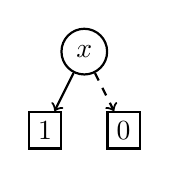
\begin{tikzpicture}
\node[circle, thick, draw] (v1) at (0,1) {$x$};
\node[rectangle, thick, draw] (v2) at (-0.5,0) {$1$};
\node[rectangle, thick, draw] (v3) at (0.5,0) {$0$};

\draw[->, thick]  (v1) edge (v2);
\draw[->, thick, dashed]  (v1) edge (v3);

\end{tikzpicture}
		$\vspace{360pt}$
	}
	$\hspace{36pt}$
	\subfloat[$\neg x$] {
		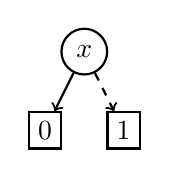
\begin{tikzpicture}
\node[circle, thick, draw] (v1) at (0,1) {$x$};
\node[rectangle, thick, draw] (v2) at (-0.5,0) {$0$};
\node[rectangle, thick, draw] (v3) at (0.5,0) {$1$};

\draw[->, thick]  (v1) edge (v2);
\draw[->, thick, dashed]  (v1) edge (v3);

\end{tikzpicture}
	}
	$\hspace{36pt}$
	\subfloat[$x_0 \wedge x_1$] {
		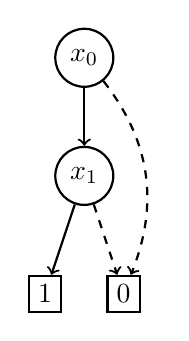
\begin{tikzpicture}
\node[circle, thick, draw] (v4) at (0,3) {$x_0$};
\node[circle, thick, draw] (v1) at (0,1.5) {$x_1$};
\node[rectangle, thick, draw] (v2) at (-0.5,0) {$1$};
\node[rectangle, thick, draw] (v3) at (0.5,0) {$0$};

\draw[->, thick]  (v1) edge (v2);
\draw[->, thick, dashed]  (v1) edge (v3);

\draw[->, thick]  (v4) edge (v1);
\draw[->, thick, dashed]  (v4) edge [bend left=30 ] (v3);

\end{tikzpicture}
	}
	$\hspace{36pt}$
	\subfloat[$x_0 \vee x_1$] {
		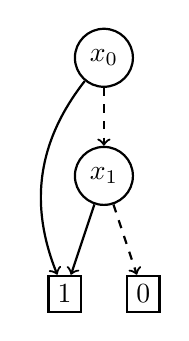
\begin{tikzpicture}
\node[circle, thick, draw] (v4) at (0,3) {$x_0$};
\node[circle, thick, draw] (v1) at (0,1.5) {$x_1$};
\node[rectangle, thick, draw] (v2) at (-0.5,0) {$1$};
\node[rectangle, thick, draw] (v3) at (0.5,0) {$0$};

\draw[->, thick]  (v1) edge (v2);
\draw[->, thick, dashed]  (v1) edge (v3);

\draw[->, thick]  (v4) edge [bend right=30 ] (v2);
\draw[->, thick, dashed]  (v4) edge (v1);

\end{tikzpicture}
	}
	
	\caption{The BDD representation of four different simple boolean functions are displayed.}
	\label{fig:bdd_examples}
\end{figure}

It is possible to represent a set of states $S \subseteq U$ from some universe $U$ by a boolean function $f : S \rightarrow \mathbb{B}$, such that $S = \{ x \in U \ | \ f(x) \}$. If $U = \mathbb{B}^n$, then $f$ is a function with signature $f : \mathbb{B}^n \rightarrow \mathbb{B}$ and so $f$ can be represented as a BDD. 

By applying this trick the state space of some program can efficiently be represented as a BDD. Suppose that the program uses a set of variable names $X = \{ x_1, \dots, x_n \}$ and we have an assignment function $v : X \rightarrow \mathbb{B}$. Then $U = \mathbb{B}^n$ can represent all possible variable assignments under $v$ and $S = \mathbb{B}^n$ represents all reachable states. Now a boolean function $f : S = \mathbb{B}^n \rightarrow \mathbb{B}$ can be given. Suppose that the program uses a transition relation $R \subseteq S \times S$. Then the same trick can be applied again to represent $R$.

We now introduce reduced ordened BDDs.

\begin{definition}
	A \emph{Reduced Ordened BDD (ROBDD)} is an ordened BDD without redundant nodes. A node $p$ is redundent if $p[0] = p[1]$.
\end{definition}

\begin{figure}
	\centering
	\subfloat[BDD with duplicate nodes] {
		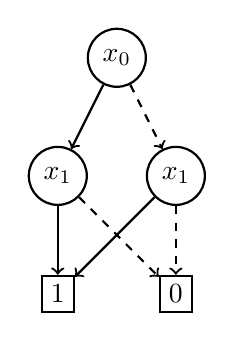
\begin{tikzpicture}
\node[circle, thick, draw] (v4) at (0.25,3) {$x_0$};
\node[circle, thick, draw] (v1) at (-0.5,1.5) {$x_1$};
\node[circle, thick, draw] (v5) at (1,1.5) {$x_1$};
\node[rectangle, thick, draw] (v2) at (-0.5,0) {$1$};
\node[rectangle, thick, draw] (v3) at (1,0) {$0$};

\draw[->, thick]  (v1) edge (v2);
\draw[->, thick, dashed]  (v1) edge (v3);
\draw[->, thick]  (v4) edge (v1);
\draw[->, thick, dashed]  (v4) edge (v5);
\draw[->, thick]  (v5) edge (v2);
\draw[->, thick, dashed]  (v5) edge (v3);

\end{tikzpicture}
		$\vspace{360pt}$
	}
	$\hspace{36pt}$
	\subfloat[BDD with a redundant node] {
		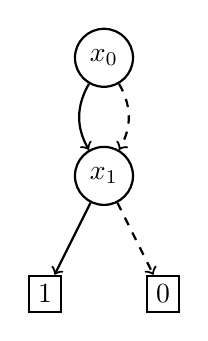
\begin{tikzpicture}
\node[circle, thick, draw] (v4) at (0.25,3) {$x_0$};
\node[circle, thick, draw] (v1) at (0.25,1.5) {$x_1$};

\node[rectangle, thick, draw] (v2) at (-0.5,0) {$1$};
\node[rectangle, thick, draw] (v3) at (1,0) {$0$};

\draw[->, thick]  (v1) edge (v2);
\draw[->, thick, dashed]  (v1) edge (v3);
\draw[->, thick]  (v4) edge [bend right=30] (v1);
\draw[->, thick, dashed]  (v4) edge [bend left=30] (v1);


\end{tikzpicture}
	}
	$\hspace{36pt}$
	\subfloat[Reduced Ordened BDD] {
		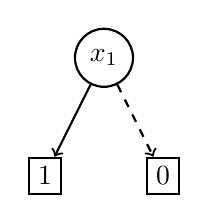
\begin{tikzpicture}

\node[circle, thick, draw] (v1) at (0.25,1.5) {$x_1$};

\node[rectangle, thick, draw] (v2) at (-0.5,0) {$1$};
\node[rectangle, thick, draw] (v3) at (1,0) {$0$};

\draw[->, thick]  (v1) edge (v2);
\draw[->, thick, dashed]  (v1) edge (v3);



\end{tikzpicture}
	}
	
	\caption{Three BDD representations of the boolean function $(x_0 \wedge x_1) \vee (\overline{x_0} \wedge x_1)$ (left representation), which is equivalent to $x_1$ (right representation). The rightmost BDD is obtained by removing duplicates and redundant nodes.}
	\label{fig:bdd_reductions}
\end{figure}

Figure \ref{fig:bdd_reductions} shows examples of BDDs that have duplicate nodes an redundant nodes. In Figure \ref{fig:bdd_reductions} all three BDDs are equivalent to each other, only the rightmost one is reduced and ordened. 

\section{Sequential BDD operations}
BDD operations use two tables, namely a \emph{Unique Table} and a \emph{Computed Table}. The unique table is used to store BDD nodes and is necessary to ensure that there are no duplicate nodes. The unique table is usually implemented as a hash table. The computed table acts as a cache. Most of the BDD operations are recursively defined, and the subresults are stored in the computed table. Before performing recursive calls the operations can check if the operation has been done before.

Most BDD operations are based on a concept called Shannon decomposition \cite{dijk2012parallelization}, which is defined below.

\begin{definition}[Restriction]
	Let $X = \{ x_1, \dots, x_n \}$ be a set of variable names and $\phi(x_1, \dots, x_n)$ a boolean formula (i.e. with codomain $\mathbb{B}$). Then the \emph{restriction} of $v$ to $x_i \in X$ in $\phi$, denoted by $\phi_{x_i=v}$, is defined by 
	\begin{equation}
		\phi_{x_i=v} \equiv \phi(x_1, \dots, x_{i - 1}, v, x_{i + 1}, \dots, x_n)
	\end{equation}
\end{definition}

\begin{definition}[Shannon Decomposition]
	Let $X = \{ x_1, \dots, x_n \}$ be a set of variable names and $\phi(x_1, \dots, x_n)$ a boolean formula (i.e. with codomain $\mathbb{B}$). Then the \emph{Shannon decomposition} of $\phi$ along $x \in X$ is defined as $\psi = (x \wedge \phi_{x=1}) \vee (\overline{x} \wedge \phi_{x=0})$ such that $\phi \equiv \psi$. 
\end{definition}

Many BDD operations are implemented by taking some variable $x$ and recursively calculating the results of the subproblems $\phi_{x=0}$ and $\phi_{x=1}$ by making a BDD of the Shannon decomposition of $\phi$ along $x$. 

Furthermore existential quantification and substitution is needed to implement the \emph{relational product} operation.

\begin{definition}[Existential Quantification]
	Let $X = \{ x_1, \dots, x_n \}$ be a set of variable names and $\phi$ be a boolean function. Take $x \in X$. Then existential quantification is defined as $\exists x \phi = \phi_{x=0} \vee \phi_{x=1}$. Take $X' = \{ x'_1, \dots, x'_m \} \subseteq X$. Then $\exists X' \phi \equiv \exists x'_1, \dots, \exists x'_m \phi$.
\end{definition}

\begin{definition}[Substitution]
	Let $X = \{ x_1, \dots, x_n \}$ be a set of variable names and $\phi$ be a boolean function. Take $x_i, y \in X$. Then substitution is defined by:
	\begin{equation}
		\phi[x_i \gets y] \equiv \phi(x_1, \dots, x_{i - 1}, y, x_{i + 1}, \dots, x_n)
	\end{equation}
	Now consider two sets $Y = \{ y_1, \dots, y_m \} \subseteq X$ and $Z = \{ z_1, \dots, z_m \} \subseteq X$ of variable names. Then $\phi[Y \gets Z]$ is defined as:
	\begin{equation}
		\phi[Y \gets Z] \equiv (((\phi[y_1 \gets z_1])[y_2 \gets z_2]) \dots [y_m \gets z_m])
	\end{equation}
\end{definition}

The following two sections describe the two basic BDD operations \texttt{ite} and \texttt{relprod}.

\subsection{The \texttt{ite} operation}
Many BDD operations can be expressed with the \texttt{ite} operation (which stands for if-then-else). This operation is specified as \cite{dijk2012parallelization}:
\begin{equation}
	\texttt{ite}(A, B, C) \equiv (A \wedge B) \vee (\overline A \wedge C)
\end{equation}
where $A, B, C$ are boolean formulas. Table \ref{tab:ite} shows a number of boolean formulas expressed with the \texttt{ite} operation.

\begin{table}[ht]
	\centering
	\begin{tabular}{| c | l |}
		\hline
		Operator & ITE \\ 
		\hline 
		$F \wedge G$ & $\texttt{ite}(F, G, 0)$ \\
		$F \vee G$ & $\texttt{ite}(F, 1, G)$ \\
		$F \oplus G$ & $\texttt{ite}(F, \overline G, G)$ \\
		$\neg (F \wedge G)$ & $\texttt{ite}(F, \overline G, 1)$ \\
		$\neg (F \vee G)$ & $\texttt{ite}(F, 0, \overline G)$ \\
		$F \rightarrow G$ & $\texttt{ite}(F, G, 1)$ \\
		$F \leftarrow G$ & $\texttt{ite}(F, 1, \overline G)$ \\
		$F \leftrightarrow G$ & $\texttt{ite}(F, G, \overline G)$ \\
		$\overline F \wedge G$ & $\texttt{ite}(F, 0, G)$ \\
		$F \wedge \overline G$ & $\texttt{ite}(F, \overline G, 0)$ \\
		\hline
	\end{tabular}
	\caption{This table shows several boolean formulas expressed with the \texttt{ite} operation. This table is taken from \cite{dijk2012parallelization}.}
	\label{tab:ite}
\end{table}

\begin{figure}
	\centering
	\begin{algorithm}[H]
		\SetStartEndCondition{ }{}{}%
		\SetKwProg{Fn}{bdd}{\string:}{}
		\SetKwFunction{fun}{ite}
		\SetKw{KwTo}{in}\SetKwFor{For}{for}{\string:}{}%
		\SetKwIF{If}{ElseIf}{Else}{if}{}{elif}{else}{}%
		\SetKwFor{While}{while}{:}{fintq}%
		\SetKw{test}{in}{}%
		\AlgoDontDisplayBlockMarkers\SetAlgoNoEnd\SetAlgoNoLine%

		\Fn{\fun{\textbf{bdd} $A$, \textbf{bdd} $B$, \textbf{bdd} $C$}} {
			\textbf{if} $A=1$ \textbf{return} $B$ \\
			\textbf{if} $A=0$ \textbf{return} $C$ \\
			\textbf{if} $\texttt{in-cache}(A, B, C)$ \textbf{return} $\texttt{cache-lookup}(A,B,C)$ \\
			$x \gets \texttt{min}(\texttt{var}(A), \texttt{var}(B), \texttt{var}(C))$ \\
			$R_{low} \gets \texttt{ite}(\texttt{low}(A, x), \texttt{low}(B, x), \texttt{low}(C, x))$ \\
			$R_{high} \gets \texttt{ite}(\texttt{high}(A, x), \texttt{high}(B, x), \texttt{high}(C, x))$ \\
			$R \gets \texttt{mk}(x, R_{low}, R_{high})$ \\
			$\texttt{add-to-cache}(A, B, C, R)$ \\
			\Return{$R$}
		}
	\end{algorithm}

	\caption{The (sequential) implementation of the \texttt{ite} operation.}
	\label{fig:ite_seq}
\end{figure}

The implementation of the \texttt{ite} function is given in Figure \ref{fig:ite_seq}. Instead of taking three boolean formulas, the implementation takes their BDD representations. The \texttt{in-cache}, \texttt{cache-lookup}, and \texttt{add-to-cache} functions tests if the BDD is in the computed table, gets the BDD from the computed table and adds the BDD to the computed table, respectively.

The operations \texttt{low} and \texttt{high} calculate the \emph{cofactor} of their first operand. These two functions are specified as follows:
\begin{equation}
	\texttt{low}(F, x) \equiv F_{x=0}
\end{equation}
\begin{equation}
	\texttt{high}(F, x) \equiv F_{x=1}
\end{equation}

The \texttt{mk} function creates a new BDD node and adds it to the unique table.

\subsection{The \texttt{relprod} operation}
Binary Decision Diagrams are used in symbolic model checking. An important model checking algorithm is the \emph{reachability} algorithm, which determines the set of all reachable program states, given an initial state and a transition relation. 

Burch et al. \cite{burch1994symbolic} used the \emph{relational product} operation to implement the reachability algorithm, where both the initial state and the transition relation function are represented by boolean functions. The relational product has the form: 
\begin{equation}
	\texttt{relprod}(A, B, X) \equiv \exists X. (A \wedge B)
	\label{eqn:relprod}
\end{equation}
where $X$ is a set of variables and $A, B$ are boolean functions.

Let $X = \{ x_1, \dots, x_n \}$ be a set of variable names. Suppose that $\phi(x_1, \dots, x_n) \equiv \phi(X)$ represent a set of states and $\psi(x_1, \dots, x_n, x'_1, \dots, x'_n) \equiv \psi(X, X')$ represent the transition relation. Then \texttt{relprod} \ref{eqn:relprod} is used to calculate the next set of states $\phi'(X)$ by:
\begin{equation}
	\phi'(X') \equiv \exists X. (\phi(X) \wedge \psi(X, X')) \equiv \texttt{relprod}(\phi(X), \psi(X, X'), X)
	\label{eqn:relprod_1}
\end{equation}
\begin{equation}
	\phi'(X) \equiv \phi'(X')[X' \gets X]
	\label{eqn:relprod_2}
\end{equation}
Note that $\phi(X)$ is used in \ref{eqn:relprod_1} so that the successors calculated by $\psi(X, X')$ are limited to states represented by $\phi(X)$. Then all variable names of $X$ are abstracted, so that only variable names in $X'$ remain. The last step, which is performed in \ref{eqn:relprod_2}, is to rename all variable names from $X'$ to $X$. This is done by applying substitution. The result is the set of states $\phi'(X)$ reachable from $\phi(X)$ by applying the transition relation.

\begin{figure}
	\centering
	\begin{algorithm}[H]
		\SetStartEndCondition{ }{}{}%
		\SetKwProg{Fn}{bdd}{\string:}{}
		\SetKwFunction{fun}{relprod}
		\SetKw{KwTo}{in}\SetKwFor{For}{for}{\string:}{}%
		\SetKwIF{If}{ElseIf}{Else}{if}{}{elif}{else}{}%
		\SetKwFor{While}{while}{:}{fintq}%
		\SetKw{test}{in}{}%
		\AlgoDontDisplayBlockMarkers\SetAlgoNoEnd\SetAlgoNoLine%

		\Fn{\fun{\textbf{bdd} $A$, \textbf{bdd} $B$, $X$}} {
			\textbf{if} $A=1 \wedge B=1$ \textbf{return} $1$ \\
			\textbf{if} $A=0 \vee B=0$ \textbf{return} $0$ \\
			\textbf{if} $\texttt{in-cache}(A, B, X)$ \textbf{return} $\texttt{cache-lookup}(A, B, X)$ \\
			$x \gets \texttt{min}(\texttt{var}(A), \texttt{var}(B))$ \\
			$R_{low} \gets \texttt{relprod}(\texttt{low}(A, x), \texttt{low}(B, x), X)$ \\
			$R_{high} \gets \texttt{relprod}(\texttt{high}(A, x), \texttt{high}(B, x), X)$ \\

			\If{$x \in X$} {
				$R \gets \texttt{ite}(R_{low}, 1, R_{high})$
			}
			\Else {
				$R \gets \texttt{mk}(x, R_{low}, R_{high})$ \\
			}
			
			$\texttt{add-to-cache}(A, B, X, R)$ \\
			\Return{$R$}
		}
	\end{algorithm}

	\caption{The sequential implementation of the \texttt{relprod} operation.}
	\label{fig:relprod_seq}
\end{figure}

Figure \ref{fig:relprod_seq} shows an implementation of the \texttt{relprod} function. The implementation of \cite{dijk2012parallelization} shows that if $x \in X$ and $R_{low} = 1$ then the result $1$ can simply be returned. This algorithm however shows the essence of the relational product implementation. \cite{dijk2012parallelization} also gives a new algorithm \texttt{relprods} that is more efficient than \texttt{relprod} because it does not create BDD nodes unnecessarily.

\subsection{Sequential Reachability}
The previous section shows how the \texttt{relprod} operations can be used to calculate the next set of states $\phi'(X)$ given an initial state $\phi(X)$ and a transition relation $\psi(X, X')$. Suppose that $\phi$ and $\psi$ are represented by the BDDs $I$ and $T$, respectively. Then the implementation for the sequential reachability algorithm \texttt{reach} is given in Figure \ref{fig:reach_seq}.

\begin{figure}
	\centering
	\begin{algorithm}[H]
		\SetStartEndCondition{ }{}{}%
		\SetKwProg{Fn}{bdd}{\string:}{}
		\SetKwFunction{fun}{reach}
		\SetKw{KwTo}{in}\SetKwFor{For}{for}{\string:}{}%
		\SetKwIF{If}{ElseIf}{Else}{if}{}{elif}{else}{}%
		\SetKwFor{While}{while}{:}{fintq}%
		\SetKw{test}{in}{}%
		\AlgoDontDisplayBlockMarkers\SetAlgoNoEnd\SetAlgoNoLine%

		\Fn{\fun{\textbf{bdd} $I$, \textbf{bdd} $T$, $X$, $X'$}} {
			$R \gets I$ \\
			$P \gets 0$ \\
			\While{$R \not = P$} {
				$N \gets \texttt{relprod}(R, T, X)$ \\
				$N \gets N[X' \gets X]$ \\
				$P \gets R$ \\
				$R \gets \texttt{ite}(R, 1, N)$
			}
			\Return{$R$}
		}
	\end{algorithm}

	\caption{The sequential implementation of the reachability operation.}
	\label{fig:reach_seq}
\end{figure}

In every iteration of the while loop (lines 4 to 8) the set of next states (represented by $N$) is calculated from the current set of states (represented by $R$) and the two are combined by using the \texttt{ite} equivalent of the $\vee$ operation. Suppose that $\phi_0(X) \equiv \phi(X)$ and $\phi_{i+1}(X) \equiv \phi'_i(X) \vee \phi_i(X)$. Then the while loop at line 4 terminates when $\phi_{i} = \phi_{i+1}$ after $i+1$ iterations. At that point a fixpoint is reached and the BDD representation of $\phi_{i+1}$, which is the $R$ at line 9, is returned.

\section{Garbage Collection}
After performing BDD operations it may happen that some nodes become unused due to reduction. If the memory needs to be used efficiently, then \emph{garbage collection} is essential. The process of garbage collection removes all unused nodes from the unique table. There are several algorithms for garbage collection, which are discussed below. 

Somenzi \cite{somenzi2001efficient} pointed out that unused BDD nodes are often reused. This may have a negative impact on the performance of garbage collection, since nodes are possibly recreated. Therefore \cite{somenzi2001efficient} suggested that garbage collection should only be performend when there are enough unused nodes. Then the cost of the garbage collection algorithm can be justified.

In the next two sections the garbage collection techniques \emph{reference counter} and \emph{mark-and-sweep} are discussed.

\subsection{Reference Counting}
With reference counting, the number of references to a BDD nodes are recorded and stored in the unique table, together with the BDD node itself. Increasing and decreasing the reference counter can be done by performing a \texttt{compare-and-swap} operation on the reference counting bits of the bucket in which the corresponding BDD node is stored. 

When the reference counter of a BDD node becomes zero, then it is unused. When there are enough unused BDD nodes in the unique table, the garbage collection procedure is called, which deletes all unused BDD nodes with complexity $\mathcal{O}(n)$. Garbage collection can be made more efficient by letting the \texttt{mk} procedure reuse nodes that are currently unused. Then the expensive garbage collection procedure does not have to be called.

If reference counting is used in combination with RDMA, then updating the reference counter of a BDD may result in an extra RDMA write. Minimizing the number of RDMA calls is crucial for both performance and scalability, so we should try to combine reference counting with other BDD operations or we should try to find another garbage collection method. On the other hand, performing the actual removal of BDD nodes from the unique table can be done both individually and locally by each of the participating machines, even without the need to synchronize. 

\subsubsection{Related Work}
The parallel BDD implementations described in \cite{dijk2012parallelization} and \cite{sylvan_multicore_bdd} both use reference counting. This is justifiable since mark-and-sweep requires the entire computation to stop when garbage collection is performed and reference counting does not. This might be different in a distributed setting. 

\subsection{Mark and Sweep}
Another garbage collection scheme used in BDD manipulation is \emph{mark-and-sweep} \cite{mccarthy1960recursive}. Mark-and-sweep requires two passes. In the first pass (the marking pass), every BDD node that is referenced is marked. In the second pass (the sweeping pass) every BDD node that is not marked is removed. So every BDD node receives an extra bit in the unique table for marking and no reference counter is needed.

The advantage of mark-and-sweep is that no extra work needs to be done for garbage collection when a BDD node is referenced. All work for garbage collection is performed when the \texttt{garbage-collect} procedure is called. This may speed up BDD operations, especially when RDMA is used to implement them. 

The disadvantage of mark-and-sweep is that two passes are needed instead of one. Another disadvantage is that the entire computation stops during garbage collection. The advantages of PGAS can however be used to speed up garbage collection. Both the marking and the sweeping passes can be done in parallel. First the \texttt{garbage-collect} procedure partitions the unique table across all participating processes. In the marking pass each process takes a partition that resides in local memory. Then BDD nodes can be marked by using an RDMA \texttt{compare-and-swap} computation. In the sweep pass every process iterates over its local partition and removed every BDD node that is not marked.

\subsubsection{Lazy Sweeping}
A variant on mark-and-sweep is \emph{lazy sweeping}, also called \emph{mark-and-don't-sweep}. In lazy sweeping each bucket in the hash table is marked with some bit $b$ as either black ($b=0$) or white ($b=1$). When the load-factor $\alpha$ reaches some treshold, \texttt{garbage-collect} is called, which flips the interpretation of $b$. So $b=1$ becomes black and $b=0$ becomes white. This means that every bucket in the hash table (temporarily) becomes white. A single marking pass follows that makes all referenced buckets black again. With this technique only a single marking pass is needed instead of two passes. The marking pass can be performed in parallel by doing the same trick as in mark-and-sweep.

\subsubsection{Related Work}
The BDDNOW package \cite{bddnow}, which is a parallel BDD package, uses mark-and-sweep for garbage collection. The researchers argued that keeping track of reference counts in a distributed environment is costly, so mark-and-sweep should be used instead.

In \cite{chen1997breadth} hybrid breath-first and depth-first algorithms are given for BDD construction. The researchers preferred mark-and-sweep over reference counting because mark-and-sweep uses less memory. Mark-and-sweep can be implemented by adding a single bit to the unique table, and reference counting requires more bits. 

\section{Parallel BDD operations}
A parallel version of the \texttt{ite} and \texttt{relprod} operations is given in \cite{dijk2012parallelization} and \cite{sylvan_multicore_bdd}. The unique table and the computed table are implemented using the lockless hash table described in \cite{so73119}. Furthermore the recursive calls in Figures \ref{fig:ite_seq} and \ref{fig:relprod_seq} are done in parallel by using a work stealing framework. The implementation of \cite{dijk2012parallelization} uses the Wool framework \cite{faxen2010efficient} and the implementation of \cite{sylvan_multicore_bdd} uses Lace \cite{dijk2013lace}. 

\subsection{Parallel Reachability}
Unfinished..

\bibliography{References}
\bibliographystyle{plain}

\end{document}